\documentclass[a4paper,11pt] {article}
\hfuzz=100pt 
%\documentclass[a4paper,article,oneside,10pt]{memoir}
\usepackage[latin1]{inputenc}
\usepackage[T1]{fontenc}
%\usepackage[lucidasmallscale, nofontinfo]{lucimatx}
%\usepackage{times}
\usepackage{graphicx}
\usepackage{longtable}
\usepackage{here}
\usepackage{ctable}
\usepackage{pdflscape}
\usepackage{pst-tree}
\usepackage{longtable}
\usepackage{multirow}
\usepackage{dcolumn}
\usepackage{Sweave}
\usepackage{lscape}
\usepackage{geometry}
\usepackage{graphicx}
\usepackage{subfig}
\usepackage{caption}
%\usepackage[pdftex,bookmarks=true,bookmarksnumbered=true,
%            hypertexnames=false,breaklinks=true,
%            linkbordercolor={0 0 1}]{hyperref}

%--------------

%
%\usepackage{fancyhdr}
%\pagestyle{empty}
%\pagestyle{fancy}
%\fancyhf{}
%%\renewcommand{\chaptermark}[1]{\markboth{\bsc{\chaptername~\thechapter{} :} #1}{}}
%%\renewcommand{\sectionmark}[1]{\markright{\thesection{} #1}}
%%\lfoot{Confidential, for the exclusive use of DMC members}
%%\renewcommand{\footrulewidth}{0.4pt}
%%\renewcommand{\headrulewidth}{0.4pt}
%%\renewcommand{\thepage}{\arabic{\page}}
%\setcounter{tocdepth}{5} % Dans la table des matieres
%\setcounter{secnumdepth}{5} % Avec un numero.
%%\mainmatter
%\pagenumbering{arabic}\setcounter{page}{1}
%\rhead{\thepage}
%\lhead{\leftmark}
%%\renewcommand{\thesection}{\Roman{section}}
%%\renewcommand{\thesection}{\Roman{section}}
%%\renewcommand{\thesection}{\Roman{section}}
%%\renewcommand{\thesubsection}{\thesection .\Alph{subsection}}
%
%--------------
\begin{document}
\title{Rapport  d'analyses statistiques}
\author{Axelle Dupont, sbim, Hopital Saint Louis, Paris}
\date\today

%------------------------------------------------------------






%-------------------------------------------------------------





\Sconcordance{concordance:Rapport.tex:Rapport.Rnw:%
1 109 1 1 50 4 1 1 9 69 0 1 2 1 9 16 0 1 2 1 1 1 9 129 0 1 2 2 1 1 9 58 %
0 1 2 8 1 2 12 1 11 7 1 2 2 10 1 2 2 10 1 1 4 8 1 2 2 11 1 2 2 5 1 1 4 %
14 1 1 4 7 1 1 4 8 1 1 4 4 1 1 4 12 1 1 5 5 1 1 6 7 1 1 11 8 1}



\setkeys{Gin}{width=1\textwidth}
\maketitle

%\pagestyle{protoc}
\tableofcontents
\pagebreak[4]
\listoftables
\listoffigures
%\SweaveOpts{eval=TRUE,echo=false,fig=TRUE}


\pagebreak[4]
%\chapter{Objectif}

\section{Objectives}

The primary objective of the study was to assess the survival, the risk of relapse and GVHD  of patients who underwent allogenic sterm-cell transplantation (alloSCT) for aggressive T-cell lymphomas. 
The second objective was to determine the variables associated with these outcomes.

\section{Methods}

A retrospective analysis was conducted. A descriptive analysis of the variables recorded was perfomed.Different endpoints were defined : death, Event Free Survival (EFC), GRFS. GRFS was defined as death,progression/relapse,  grade 3-4 acute GVHD or extensive chronic GVHD.

Survival curves were estimated using Kaplan-Meier product-limit estimator.
Competing risk survival analysis methods were applied to estimate the cumulative incidence (CIF) of developing events over time from alloSCT. These methods allow for the fact that a patient may experience an event which is different from that of interest. These events are known as competing risk events, and may preclude the onset of the event of interest, or may modify the probability of the onset of that event.In particular, a transplanted patient may die before a relapse occurs. 

Factors associated with overall sur-vival were analyzed using Cox proportional hazards models. The proportional hazards assumption was checked by examination of Schoenfeld residuals. Occurence of a grade 3-4 acute GVHD or chronic GVHD was treated as a time dependent covariable.
For the different endpoints, univariable analyses were first carried out, then a multivariable analysis was used where all factors with P-value < 0.05 in the univariable analyses were considered. If needed, factors where then sequentially removed from the adjusted model based on the AIC criteria. 
%Survival is presented as estimate and 95\% confidence interval (95\% CI).


Propensity score was constructed, excluded patients that cannot receive MAC : patients aged more that 50 years, with a karnofsky score under 70, with a previous autoSCT or with a source of graft different from BM. 


\pagebreak[4]
\section{Results}





\subsection{Descriptive results}
 285 patients were initially selected.We excluded 1 patient that underwent two alloSCT. The final analysis was perfomed on 284 patients and 284 grafts.
 \subsubsection{Patients characteristics}
% latex table generated in R 3.4.4 by xtable 1.8-2 package
% Tue Jun 19 12:16:14 2018
\begin{longtable}{llll}
  \hline
Parameters & Values & N & Statistics* \\ 
  \hline
 &  & 284 &  \\ 
  Patient sex & Female & 93 & 32.75 \% \\ 
   & Male & 191 & 67.25 \% \\ 
  Age at diagnosis &  & 284 & 46.5 [36;55] (15;68) \\ 
  Stage at diagnosis & I & 13 & 6.47 \% \\ 
   & II & 17 & 8.46 \% \\ 
   & III & 45 & 22.39 \% \\ 
   & IV & 126 & 62.69 \% \\ 
   & NA & 83 &  \\ 
  Subtypes & AITL & 82 & 28.87 \% \\ 
   & ALCL ALK- & 20 & 7.04 \% \\ 
   & ALCL ALK? & 2 & 0.7 \% \\ 
   & ALCL ALK+ & 21 & 7.39 \% \\ 
   & ATLL & 16 & 5.63 \% \\ 
   & EATL & 3 & 1.06 \% \\ 
   & HS & 12 & 4.23 \% \\ 
   & LGL & 1 & 0.35 \% \\ 
   & NK leukemia & 1 & 0.35 \% \\ 
   & NK/T nasal & 16 & 5.63 \% \\ 
   & NOS & 110 & 38.73 \% \\ 
  Subtypes & NOS & 110 & 38.73 \% \\ 
   & AITL & 82 & 28.87 \% \\ 
   & ALCL & 43 & 15.14 \% \\ 
   & ATLL & 16 & 5.63 \% \\ 
   & NK/T nasal & 16 & 5.63 \% \\ 
   & Others & 17 & 5.99 \% \\ 
  Centres & angers & 8 & 2.82 \% \\ 
   & Becquerel[941] & 4 & 1.41 \% \\ 
   & C.H.R.U Brest[659] & 2 & 0.7 \% \\ 
   & caen & 4 & 1.41 \% \\ 
   & CHU clermond ferrand & 7 & 2.46 \% \\ 
   & Geneve & 6 & 2.11 \% \\ 
   & Gustave Roussy[666] & 3 & 1.06 \% \\ 
   & H A Michallon[270] & 5 & 1.76 \% \\ 
   & H Bretonneau[272] & 3 & 1.06 \% \\ 
   & H Charles Nicolle[932] & 1 & 0.35 \% \\ 
   & H Claude Huriez[277] & 8 & 2.82 \% \\ 
   & H de l`ARCHET I[523]nice & 3 & 1.06 \% \\ 
   & H E Herriot[671] & 5 & 1.76 \% \\ 
   & H Haut-Leveque[267] & 31 & 10.92 \% \\ 
   & H Hautepierre[672] & 11 & 3.87 \% \\ 
   & H Jean Minjoz[233] & 5 & 1.76 \% \\ 
   & H La Miletrie[264] & 5 & 1.76 \% \\ 
   & H Mondor Hematol[252] & 4 & 1.41 \% \\ 
   & H Necker[160] & 9 & 3.17 \% \\ 
   & H Percy[665] & 4 & 1.41 \% \\ 
   & H Purpan[624] & 8 & 2.82 \% \\ 
   & H Sud/Pontchaillou[661] & 7 & 2.46 \% \\ 
   & H Sud[955] & 1 & 0.35 \% \\ 
   & Hotel Dieu[253] & 32 & 11.27 \% \\ 
   & liege & 8 & 2.82 \% \\ 
   & limoges & 3 & 1.06 \% \\ 
   & montpellier & 10 & 3.52 \% \\ 
   & nancy & 1 & 0.35 \% \\ 
   & Paoli Calmettes[230] & 39 & 13.73 \% \\ 
   & Pellegrin-Enfants[978] & 1 & 0.35 \% \\ 
   & Pitie-Salpetrriere[262] & 8 & 2.82 \% \\ 
   & St Antoine[775] & 10 & 3.52 \% \\ 
   & St Etienne[250] & 4 & 1.41 \% \\ 
   & St Louis[207] & 24 & 8.45 \% \\ 
   &  & 0 & 0 \% \\ 
   \hline
\hline
\caption{Patients characteristics} 
\label{tab:condi}
\end{longtable} \subsubsection{Treatments before alloSCT}
% latex table generated in R 3.4.4 by xtable 1.8-2 package
% Tue Jun 19 12:16:15 2018
\begin{longtable}{llll}
  \hline
Parameters & Values & N & Statistics* \\ 
  \hline
 &  & 284 &  \\ 
  Previous auto & No & 191 & 67.25 \% \\ 
   & Yes & 93 & 32.75 \% \\ 
   Programme auto allo & No & 257 & 90.49 \% \\ 
   & Yes & 27 & 9.51 \% \\ 
  First graft relapse & No & 219 & 77.11 \% \\ 
   & Yes & 65 & 22.89 \% \\ 
   \hline
\hline
\caption{Treatments before alloSCT} 
\label{tab:avtg}
\end{longtable}\pagebreak
 \subsubsection{Transplant conditions}
% latex table generated in R 3.4.4 by xtable 1.8-2 package
% Tue Jun 19 12:16:15 2018
\begin{longtable}{llll}
  \hline
Parameters & Parameters & N & n(\%) med[Q1;Q3](min,max) \\ 
  \hline
 &  & 284 &  \\ 
  Age at graft &  & 284 & 49.5 [38;57] (16;69) \\ 
  Donor age &  & 263 & 28 [18;39] (1;54) \\ 
  Donor sex & Female & 114 & 40.71 \% \\ 
   & Male & 166 & 59.29 \% \\ 
   & NA & 4 &  \\ 
  Delay diagnosis and allo SCT &  & 284 & 378.5 [213.2;710.8] (89;9684) \\ 
  >12 months delay & NO & 149 & 52.46 \% \\ 
   & Yes & 135 & 47.54 \% \\ 
  Disease status at transplant & CR & 175 & 61.84 \% \\ 
   & PR & 76 & 26.86 \% \\ 
   & PD & 32 & 11.31 \% \\ 
   & NA & 1 &  \\ 
  Disease status at transplant & CR (?) & 7 & 2.47 \% \\ 
   & CR1 & 94 & 33.22 \% \\ 
   & CR2 & 61 & 21.55 \% \\ 
   & CR3 & 13 & 4.59 \% \\ 
   & PD & 32 & 11.31 \% \\ 
   & PR (?) & 13 & 4.59 \% \\ 
   & PR1 & 39 & 13.78 \% \\ 
   & PR2 & 18 & 6.36 \% \\ 
   & PR3 & 5 & 1.77 \% \\ 
   & PR4 & 1 & 0.35 \% \\ 
   & NA & 1 &  \\ 
  Karnofsky score &  & 263 & 90 [80;100] \\ 
  Karnofsky score & 100 & 92 & 34.98 \% \\ 
   & 40 & 1 & 0.38 \% \\ 
   & 50 & 4 & 1.52 \% \\ 
   & 60 & 1 & 0.38 \% \\ 
   & 70 & 9 & 3.42 \% \\ 
   & 80 & 70 & 26.62 \% \\ 
   & 90 & 86 & 32.7 \% \\ 
   & NA & 21 &  \\ 
  Karnofsky score & 100 & 92 & 34.98 \% \\ 
   & Unable to carry on normal activity & 15 & 5.7 \% \\ 
   & 90-80 & 156 & 59.32 \% \\ 
   & NA & 21 &  \\ 
  No of lines before alloSCT &  & 254 & 2 [1;3] (1;9) \\ 
  No of lines before alloSCT & 1 & 73 & 28.74 \% \\ 
   & 2 & 92 & 36.22 \% \\ 
   & 3 & 65 & 25.59 \% \\ 
   & >=4 & 24 & 9.45 \% \\ 
   & NA & 30 &  \\ 
  No of lines before alloSCT & >2 & 89 & 35.04 \% \\ 
   & 1 or 2 & 165 & 64.96 \% \\ 
   & NA & 30 &  \\ 
  HLA match & HLA mismatched & 53 & 18.66 \% \\ 
   & HLA matched & 231 & 81.34 \% \\ 
  HLA match & Alternative donnors & 53 & 18.66 \% \\ 
   & Identical sibling & 128 & 45.07 \% \\ 
   & Matched unrelated & 103 & 36.27 \% \\ 
  HLA match & Identical sibling & 128 & 45.07 \% \\ 
   & Matched unrelated & 103 & 36.27 \% \\ 
   & Mismatched relative & 7 & 2.46 \% \\ 
   & Mismatched unrelated & 13 & 4.58 \% \\ 
   & Unrelated CB & 33 & 11.62 \% \\ 
  Sex of donnor/patient & Others & 205 & 73.48 \% \\ 
   & F/M & 74 & 26.52 \% \\ 
   & NA & 5 &  \\ 
  CMV serostatus of donnor/patient & neg/neg & 91 & 32.5 \% \\ 
   & Others & 189 & 67.5 \% \\ 
   & NA & 4 &  \\ 
  Source of stem cells & BM & 49 & 17.25 \% \\ 
   & CB & 33 & 11.62 \% \\ 
   & PB & 202 & 71.13 \% \\ 
  TBI & No & 161 & 56.69 \% \\ 
   & Yes & 123 & 43.31 \% \\ 
  conditioning Intensity & MAC & 106 & 38.13 \% \\ 
   & NMA & 27 & 9.71 \% \\ 
   & RIC & 145 & 52.16 \% \\ 
   & NA & 6 &  \\ 
  Conditioning & BEAM & 1 & 0.36 \% \\ 
   & BEAM + Campath & 1 & 0.36 \% \\ 
   & BU CY  & 4 & 1.42 \% \\ 
   & BU CY + FLU+ ATG & 1 & 0.36 \% \\ 
   & BU CY ATG & 1 & 0.36 \% \\ 
   & EDX ATG & 0 & 0 \% \\ 
   & ENX TBI 2gray & 1 & 0.36 \% \\ 
   & FLU ATG & 3 & 1.07 \% \\ 
   & FLU BU 1+ ATG & 3 & 1.07 \% \\ 
   & FLU BU 2 & 1 & 0.36 \% \\ 
   & FLU BU 2+ ATG & 73 & 25.98 \% \\ 
   & FLU BU 3+ ATG & 21 & 7.47 \% \\ 
   & FLU BU 4+ ATG & 10 & 3.56 \% \\ 
   & FLU BU EDX & 8 & 2.85 \% \\ 
   & FLU BU EDX +ATG & 6 & 2.14 \% \\ 
   & FLU EDX & 1 & 0.36 \% \\ 
   & FLU EDX ATG & 3 & 1.07 \% \\ 
   & FLU EDX MEL & 1 & 0.36 \% \\ 
   & FLU ENX TBI 2gray & 24 & 8.54 \% \\ 
   & FLU ENX TBI 4gray & 2 & 0.71 \% \\ 
   & FLU ENX TBI 6gray & 1 & 0.36 \% \\ 
   & FLU ENX TBI 6gray + campath & 1 & 0.36 \% \\ 
   & FLU MEL & 12 & 4.27 \% \\ 
   & FLU MEL + campath & 4 & 1.42 \% \\ 
   & FLU MEL + Campath & 1 & 0.36 \% \\ 
   & FLU MEL ATG & 1 & 0.36 \% \\ 
   & FLU MEL TBI 2gray & 1 & 0.36 \% \\ 
   & FLU TBI 2gray & 21 & 7.47 \% \\ 
   & FLU TBI 2gray ATG & 1 & 0.36 \% \\ 
   & FLU Tbi 8 gray & 1 & 0.36 \% \\ 
   & MEL 140 TBI 10 gray & 1 & 0.36 \% \\ 
   & MEL TBI VP16 & 1 & 0.36 \% \\ 
   & TB2F & 2 & 0.71 \% \\ 
   & TBI 12 gray & 1 & 0.36 \% \\ 
   & TBI 2gray & 1 & 0.36 \% \\ 
   & TBI EDX & 49 & 17.44 \% \\ 
   & TBI EDX +ATG & 11 & 3.91 \% \\ 
   & TBI EDX FLU & 5 & 1.78 \% \\ 
   & Thiotepa etoposide TBI12 gray & 1 & 0.36 \% \\ 
   & NA & 3 &  \\ 
  Cells manipulation & No & 275 & 97.86 \% \\ 
   & Yes & 6 & 2.14 \% \\ 
   & NA & 3 &  \\ 
  Depletion & No & 275 & 98.57 \% \\ 
   & Partial T depletion & 4 & 1.43 \% \\ 
   & NA & 5 &  \\ 
  No of donnors & 1 & 261 & 91.9 \% \\ 
   & 2 & 23 & 8.1 \% \\ 
   \hline
\hline
\caption{Transplant conditions} 
\label{tab:g}
\end{longtable}
\pagebreak
\subsubsection{Post-AlloSCT Response}
% latex table generated in R 3.4.4 by xtable 1.8-2 package
% Tue Jun 19 12:16:15 2018
\begin{longtable}{llll}
  \hline
Parameters & Values & N & Statistics* \\ 
  \hline
 &  & 284 &  \\ 
  Agvhd & No & 141 & 49.65 \% \\ 
   & Yes & 143 & 50.35 \% \\ 
  Agvhd grade & No aGvHD present (Grade 0) & 141 & 49.65 \% \\ 
   & Grade I & 49 & 17.25 \% \\ 
   & Grade II & 46 & 16.2 \% \\ 
   & Grade III & 24 & 8.45 \% \\ 
   & Grade IV & 17 & 5.99 \% \\ 
   & Present, grade unknown & 7 & 2.46 \% \\ 
  Cgvhd & Early death & 41 & 14.44 \% \\ 
   & no & 146 & 51.41 \% \\ 
   & yes & 97 & 34.15 \% \\ 
  Cgvhd grade & Early death (100D) & 41 & 14.44 \% \\ 
   & Extensive & 38 & 13.38 \% \\ 
   & Limited & 55 & 19.37 \% \\ 
   & No cGvh & 146 & 51.41 \% \\ 
   & grade unknown & 4 & 1.41 \% \\ 
  Engrafted & Early death (30D) & 5 & 1.76 \% \\ 
   & Engrafted & 271 & 95.42 \% \\ 
   & Lost graft & 2 & 0.7 \% \\ 
   & No engraftment & 6 & 2.11 \% \\ 
  Cause of death & HSCT-GVHd & 21 & 19.63 \% \\ 
   & HSCT-GVHd + infection & 3 & 2.8 \% \\ 
   & HSCT-infection & 27 & 25.23 \% \\ 
   & HSCT-toxicity & 4 & 3.74 \% \\ 
   & HSCT related & 3 & 2.8 \% \\ 
   & HSCT related ILD & 1 & 0.93 \% \\ 
   & HSCT related MAT & 1 & 0.93 \% \\ 
   & HSCT related MOF & 2 & 1.87 \% \\ 
   & HSCT related MVO & 1 & 0.93 \% \\ 
   & HSCT related pneumopathie interstititelle & 2 & 1.87 \% \\ 
   & HSCT related PTLD & 1 & 0.93 \% \\ 
   & HSCT related SDRA & 1 & 0.93 \% \\ 
   & Other & 1 & 0.93 \% \\ 
   & Relapse or progression of original disease & 37 & 34.58 \% \\ 
   & Secondary malignancy & 1 & 0.93 \% \\ 
   & Unknown & 1 & 0.93 \% \\ 
   & NA & 177 &  \\ 
  Best reponse after SCT & CR & 245 & 86.88 \% \\ 
   & Not evaluable & 4 & 1.42 \% \\ 
   & Not evaluated & 3 & 1.06 \% \\ 
   & PD & 14 & 4.96 \% \\ 
   & PR & 16 & 5.67 \% \\ 
   & NA & 2 &  \\ 
  Relapse/progression & Continuous progression & 28 & 9.93 \% \\ 
   & No & 217 & 76.95 \% \\ 
   & Non applicable  & 3 & 1.06 \% \\ 
   & Yes & 34 & 12.06 \% \\ 
   & NA & 2 &  \\ 
   \hline
\hline
\caption{Post-AlloSCT Response} 
\label{tab:pg}
\end{longtable}


\pagebreak[4]
\newgeometry{bmargin=1cm}
\begin{landscape}




% latex table generated in R 3.4.4 by xtable 1.8-2 package
% Tue Jun 19 12:16:15 2018
\begin{longtable}{lllllll}
  \hline
Parameters & Parameters & N & n(\%) med[Q1;Q3](min,max) & N & n(\%) med[Q1;Q3](min,max) & p \\ 
  \hline
 &  & N & Statistics* & N & Statistics* & p-value \\ 
   &  & 106 & MAC & 172 & RIC/NMA &  \\ 
  Age greffe &  & 106 & 40 [34;51] (16;64) & 172 & 54 [43;59.25] (19;69) & <0.0001 \\ 
  Nbr de lignes &  & 98 & 2 [1;3] (1;5) & 151 & 2 [2;3] (1;9) & 0.006 \\ 
  Nbr de lignes & >2 & 28 & 28.57 \% & 61 & 40.4 \% & 0.077 \\ 
   & 1 or 2 & 70 & 71.43 \% & 90 & 59.6 \% &  \\ 
   & NA & 8 &  & 21 &  &  \\ 
  Nbr de lignes & 1 & 33 & 33.67 \% & 36 & 23.84 \% & 0.053 \\ 
   & 2 & 37 & 37.76 \% & 54 & 35.76 \% &  \\ 
   & 3 & 24 & 24.49 \% & 41 & 27.15 \% &  \\ 
   & >=4 & 4 & 4.08 \% & 20 & 13.25 \% &  \\ 
   & NA & 8 &  & 21 &  &  \\ 
  
                               Autogreffe avant & 0 & 89 & 83.96 \% & 96 & 55.81 \% & <0.0001 \\ 
   & 1 & 17 & 16.04 \% & 76 & 44.19 \% &  \\ 
  Statut de la maladie & CR & 58 & 54.72 \% & 114 & 66.67 \% & 0.015 \\ 
   & PR & 39 & 36.79 \% & 36 & 21.05 \% &  \\ 
   & PD & 9 & 8.49 \% & 21 & 12.28 \% &  \\ 
   & NA & 0 &  & 1 &  &  \\ 
  Karnofsky & 100 & 39 & 38.24 \% & 53 & 33.76 \% & 0.33 \\ 
   & Unable to carry on normal activity & 8 & 7.84 \% & 7 & 4.46 \% &  \\ 
   & 90-80 & 55 & 53.92 \% & 97 & 61.78 \% &  \\ 
   & NA & 4 &  & 15 &  &  \\ 
  Stade dia & I & 5 & 6.02 \% & 8 & 6.96 \% & 0.16 \\ 
   & II & 3 & 3.61 \% & 13 & 11.3 \% &  \\ 
   & III & 17 & 20.48 \% & 28 & 24.35 \% &  \\ 
   & IV & 58 & 69.88 \% & 66 & 57.39 \% &  \\ 
   & NA & 23 &  & 57 &  &  \\ 
  Delai dia-allo (mois) &  & 106 & 289 [184;506.5] (91;6243) & 172 & 436 [264.8;874.5] (109;9684) & 0.0003 \\ 
  Delai dia allo sup a 12 mois & NO & 42 & 39.62 \% & 106 & 61.63 \% & 0.0006 \\ 
   & Yes & 64 & 60.38 \% & 66 & 38.37 \% &  \\ 
  Donneur & HLA mismatched & 13 & 12.26 \% & 40 & 23.26 \% & 0.035 \\ 
   & HLA matched & 93 & 87.74 \% & 132 & 76.74 \% &  \\ 
  Sexe d/p & Others & 80 & 76.19 \% & 121 & 72.02 \% & 0.54 \\ 
   & F/M & 25 & 23.81 \% & 47 & 27.98 \% &  \\ 
   & NA & 1 &  & 4 &  &  \\ 
  CMV d/p & neg/neg & 43 & 40.95 \% & 46 & 27.06 \% & 0.024 \\ 
   & Others & 62 & 59.05 \% & 124 & 72.94 \% &  \\ 
   & NA & 1 &  & 2 &  &  \\ 
  Origine cellule & BM & 35 & 33.02 \% & 13 & 7.56 \% & <0.0001 \\ 
   & CB & 8 & 7.55 \% & 25 & 14.53 \% &  \\ 
   & PB & 63 & 59.43 \% & 134 & 77.91 \% &  \\ 
  TBI & No & 37 & 34.91 \% & 119 & 69.19 \% &  \\ 
   & Yes & 69 & 65.09 \% & 53 & 30.81 \% &  \\ 
   \hline
\hline
\caption{Characteristics according to conditionning MAC vs MNA/RIC} 
\label{tab:tra}
\end{longtable}
\end{landscape}

\restoregeometry

\subsection{Survival analysis in all patients}

\subsubsection{Overall survival, EFS and  GRFS}


Median follow-up was 20.18 (range 0.03 to 112.83). OS at 1 year was 0.69 (95 \% 0.61 - 0.76), was 0.65 (95 \% 0.56 - 0.72) at 2 years.OS at 4 years was 0.59 (95 \% 0.49 - 0.67).
\begin{figure}[h]
\begin{center}
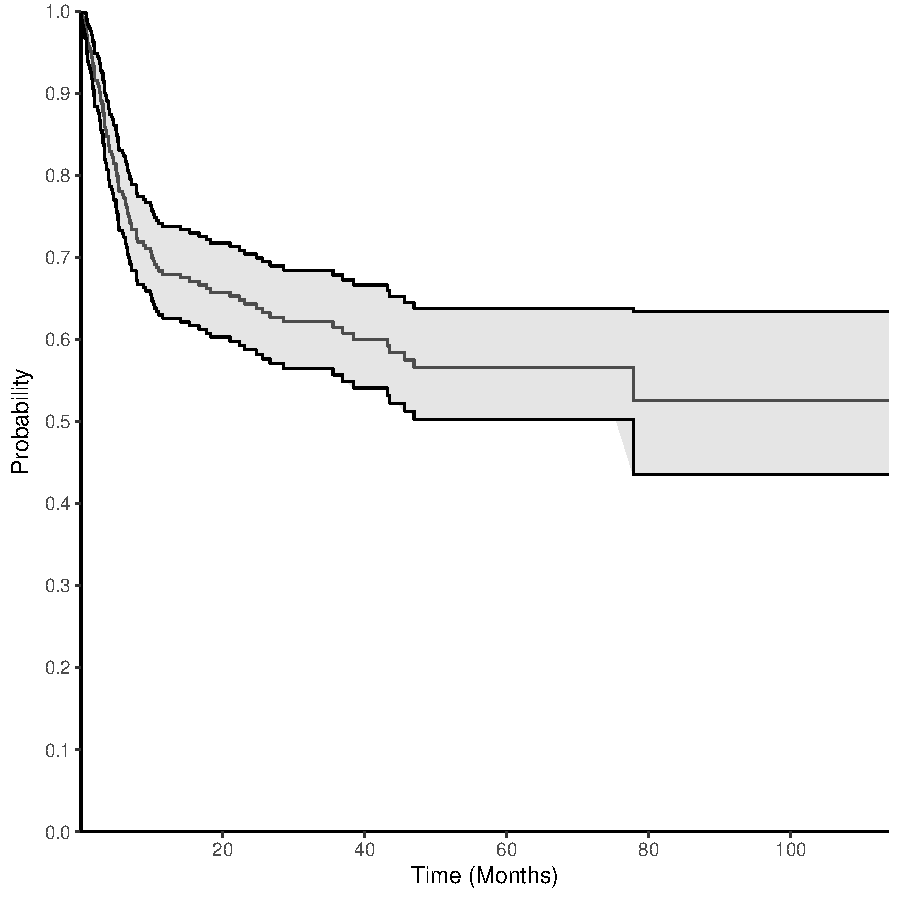
\includegraphics{Rapport-fig1}
\end{center}
\caption{Overall survival}
\label{fig1}
\end{figure}

\pagebreak
CIF for relapse/progression at 1 years was 0.19 (95 \% 0.12 - 0.25), at 2 years  0.2 (95 \% 0.13 - 0.26).
CIF for death without relapse or progression at 1 year was 0.19 (95 \% 0.12 - 0.25), at 2 years  0.21 (95 \% 0.14 - 0.28). 

\begin{figure}[h]
\begin{center}
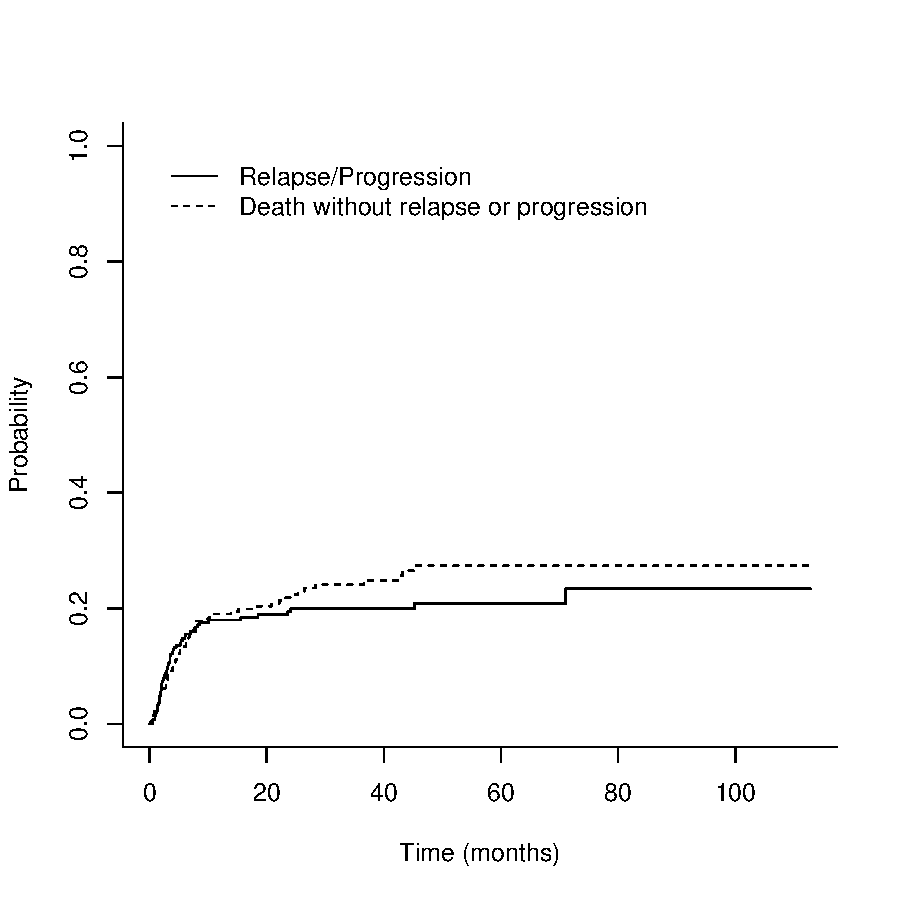
\includegraphics{Rapport-fig6}
\end{center}
\caption{CIF of relapse or progression and death without relapse or progression}
\label{fig6}
\end{figure}



\includegraphics[width=0.8\textwidth]{Z:/projetstlouis/scripts/rapport-fig6a.pdf}
\captionof{figure}{CIF of relapse or progression and death without relapse or progression according to conditionning}
\end{center}


CIF of relapse or progression with MAC at 1 year :  0.19, was 0.23 at 2 years.
CIF of relapse or progression with RIC/NMA at 1 year :  0.17, was 0.17 at 2 years.


%MAC : GVHD chronique HR 1.28 (95 \% 0.53-3.09).
%RIC : GVHD chronique HR 1.77 (95 \% 0.86-3.65).

%Interaction non significative

\pagebreak
EFS at 1 year was 0.62 (95 \% 0.55 - 0.71), was 0.59 (95 \% 0.51 - 0.68) at 2 years. EFS at 4 years was 0.55 (95 \% 0.47 - 0.65).


D�lai m�dian rechute : 94 jours.

%\begin{figure}[h]
%\begin{center}
%\end{center}
%\caption{Progression-free survival}
%\label{fig3}
%\end{figure}






GRFS at 1 year was 0.49 (95 \% 0.44 - 0.56), was 0.47 (95 \% 0.41 - 0.54) at 2 years. GRFS at 4 years was 0.43 (95 \% 0.37 - 0.5).

\begin{figure}[h]
\begin{center}
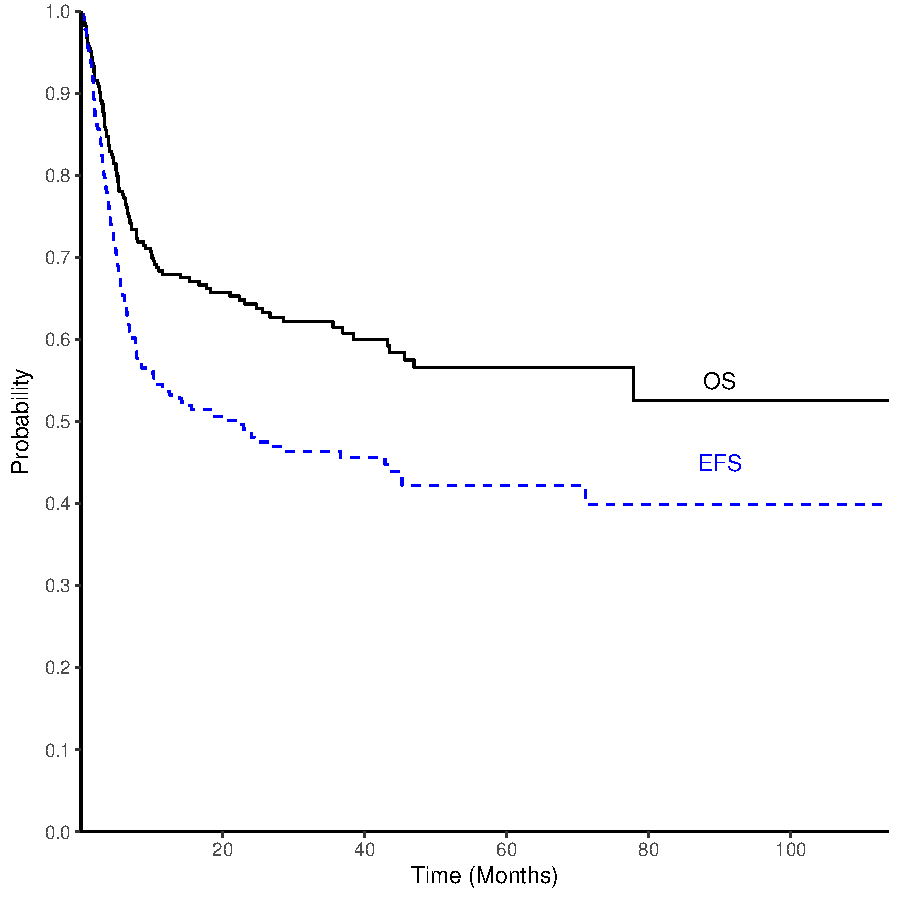
\includegraphics{Rapport-fig2}
\end{center}
\caption{EFS and GRFS}
\label{fig2}
\end{figure}





\includegraphics[width=0.8\textwidth]{Z:/projetstlouis/scripts/rapport-fig2a.pdf}
\captionof{figure}{EFS according to conditionning}
\end{center}

EFS MAC : 1 year :  0.65 (95 \% 0.56 - 0.75)
2 year :  0.59 (95 \% 0.5 - 0.7)

EFS RIC/NMA : 1 year : 0.78 (95 \% 0.72 - 0.85)
2 year :  0.73 (95 \% 0.67 - 0.8)




\pagebreak
\subsubsection{TRM and cause of death }


TRM at 1 year was 0.22 (95 \% 0.3 - 0.15), was 0.24 (95 \% 0.32 - 0.17) at 2 years. TRM at 4 years was 0.25 (95 \% 0.34 - 0.18).


\begin{figure}[h]
\begin{center}
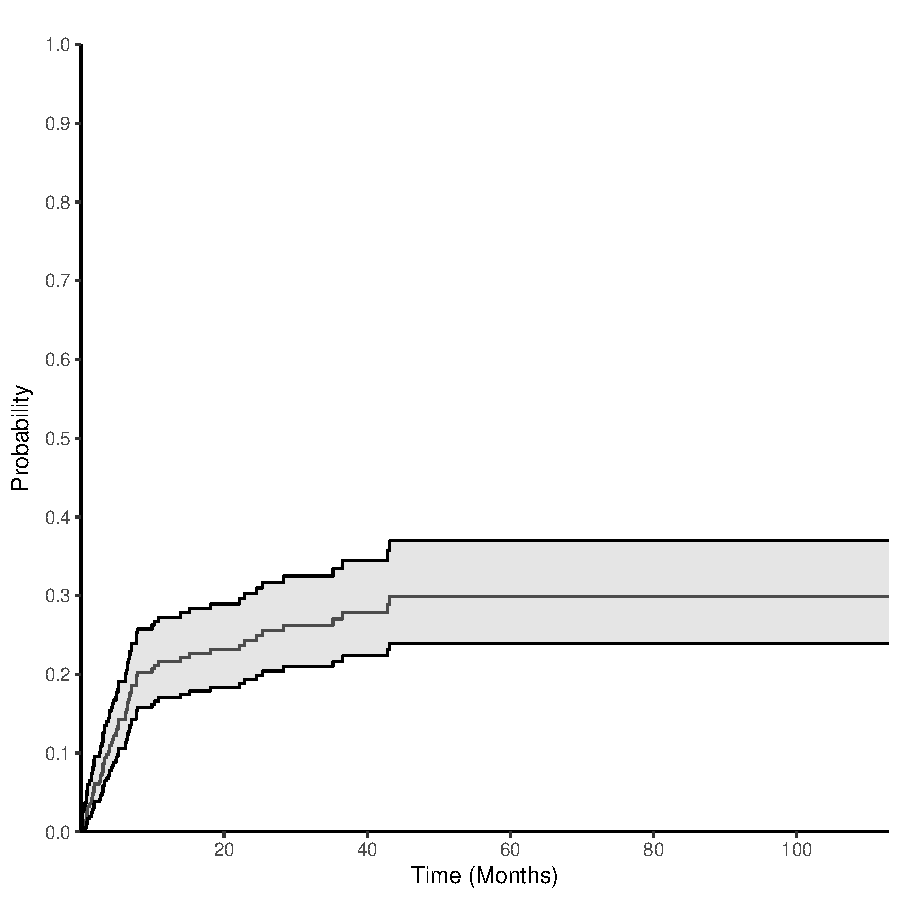
\includegraphics{Rapport-fig89}
\end{center}
\caption{TRM}
\label{fig89}
\end{figure}


\includegraphics[width=0.8\textwidth]{Z:/projetstlouis/scripts/rapport-figtrmc.pdf}
\captionof{figure}{TRM according to conditionning}
\end{center}

TRM MAC : 1 year :  0.18 (95 \% 0.26 - 0.1)
2 year :  0.2 (95 \% 0.28 - 0.11)

TRM RIC : 1 year :  0.22 (95 \% 0.28 - 0.15)
2 year :  0.26 (95 \% 0.32 - 0.18)








\begin{center}
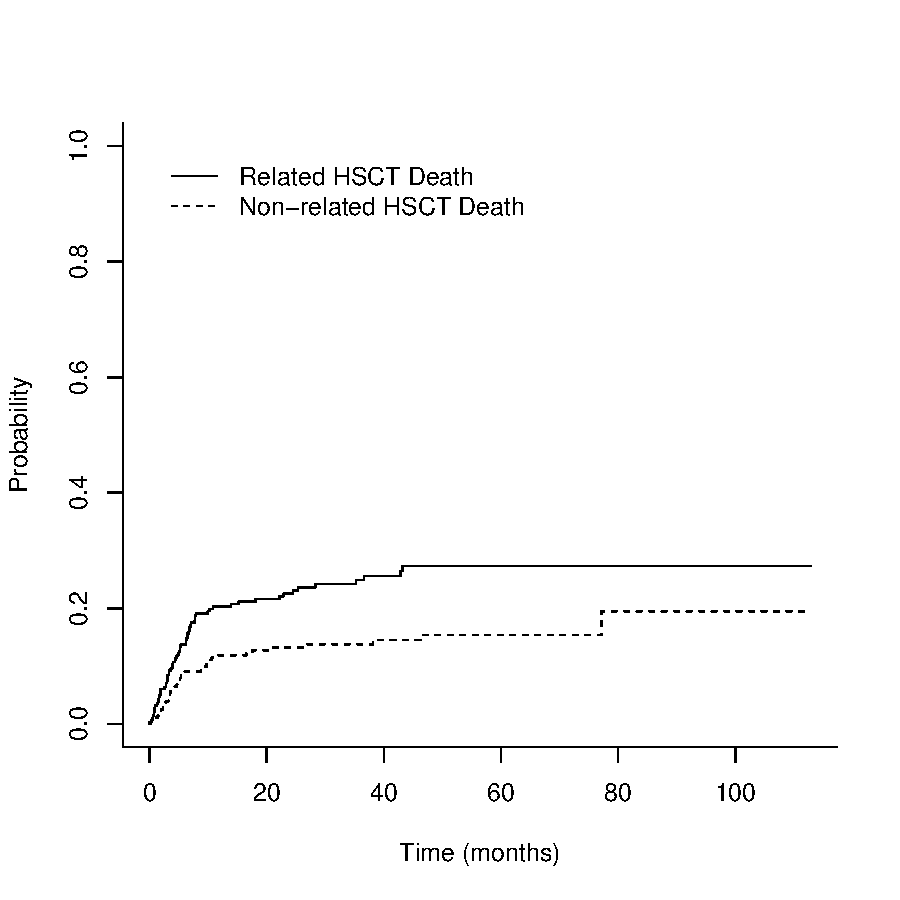
\includegraphics[width=0.8\textwidth]{Z:/projetstlouis/scripts/Rapport-fig589.pdf}
\captionof{figure}{CIF of Related HSCT Death and Non-related HSCT Death}
\end{center}



CIF for related HSCT death at 1 years was 0.2, at 2 years  0.23.
CIF for non-related HSCT Death at 1 year was 0.12, at 2 years  0.13.



\begin{center}
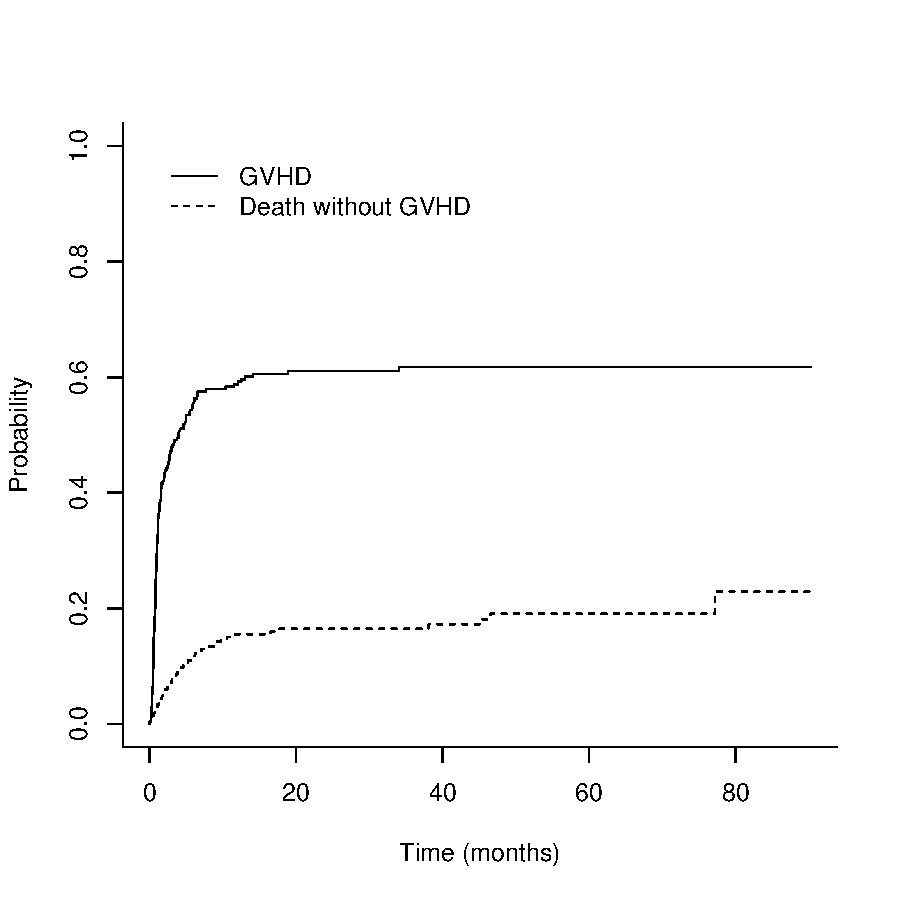
\includegraphics[width=0.8\textwidth]{Z:/projetstlouis/scripts/Rapport-fig981.pdf}
\captionof{figure}{CIF of GVHD and Death without GVHD (acute or chronic)}

\end{center}


\subsection{OS et PFS apr�s une cgvhd}


OS at 1 year after cgvhd  was 0.82 (95 \% 0.74 - 0.91), was 0.74 (95 \% 0.65 - 0.85) at 2 years


\begin{center}
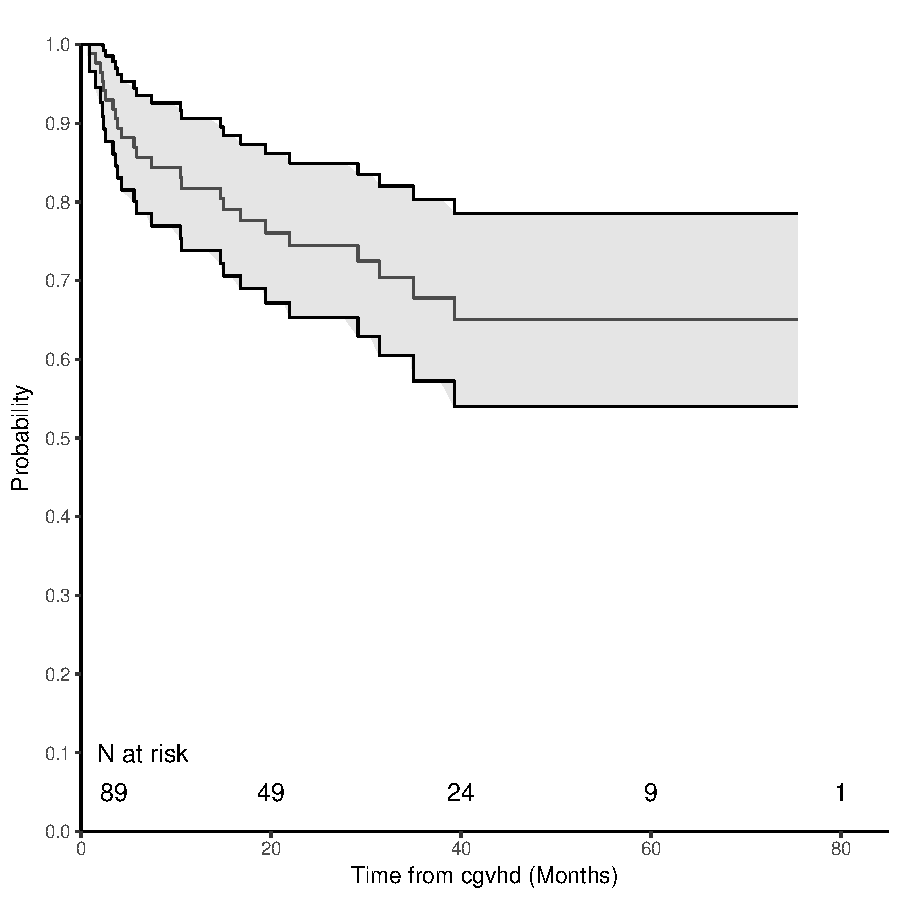
\includegraphics[width=0.8\textwidth]{Z:/projetstlouis/scripts/Rapport-figoscg.pdf}
\captionof{figure}{OS after cgvhd in cgvhd patients}

\end{center}




PFS at 1 year after cgvhd  was 0.75 (95 \% 0.64 - 0.85), was 0.66 (95 \% 0.56 - 0.77) at 2 years


\subsection{Progressive disease analysis }


OS at 6 months in the group with progressive disease at graft was 0.65 (95 \% 0.46 - 0.79).
OS at 1 year in the group with progressive disease at graft was 0.51 (95 \% 0.33 - 0.67), was 0.51 (95 \% 0.33 - 0.67) at 2 years. OS at 4 years was 0.25 (95 \% 0.08 - 0.47).




\begin{center}
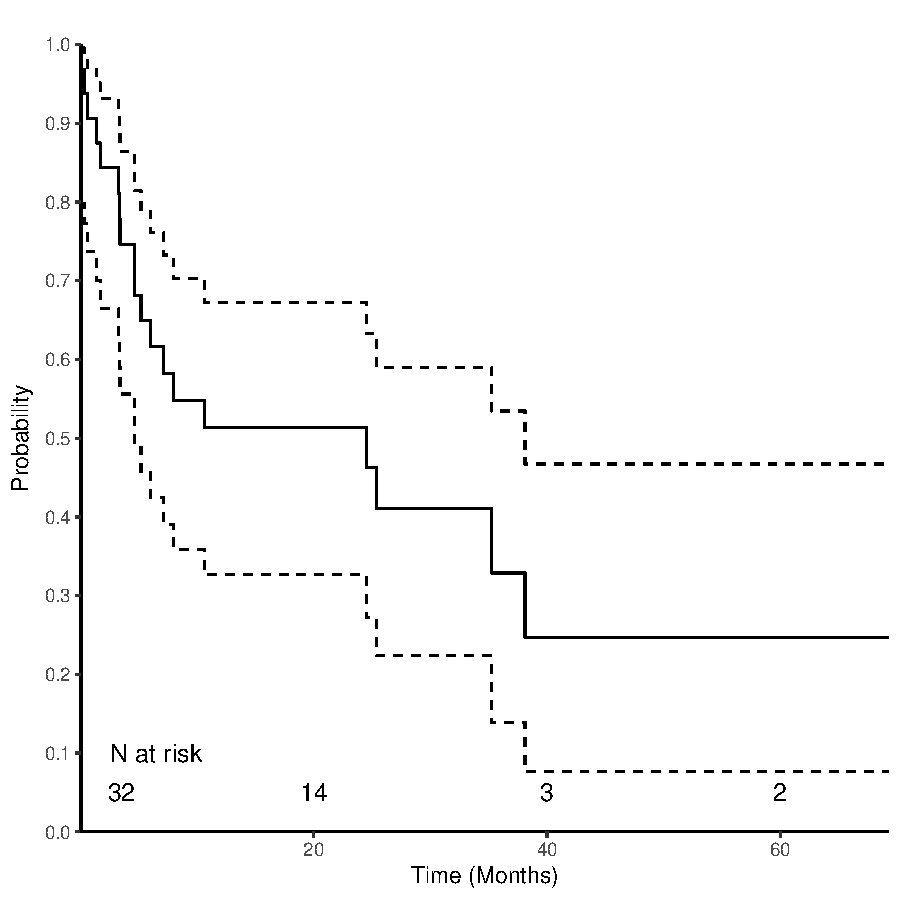
\includegraphics[width=0.8\textwidth]{Z:/projetstlouis/scripts/Rapport-figospd.pdf}
\captionof{figure}{OS in the group with progressive disease at graft}

\end{center}



TRM at 6 months in the group with progressive disease at graft was 0.18 (95 \% 0.39 - 0.08)

TRM at 1 year in the group with progressive disease at graft was 0.27 (95 \% 0.5 - 0.14), was 0.27 (95 \% 0.5 - 0.14) at 2 years. TRM at 4 years was 0.54 (95 \% 0.81 - 0.3).


\begin{center}
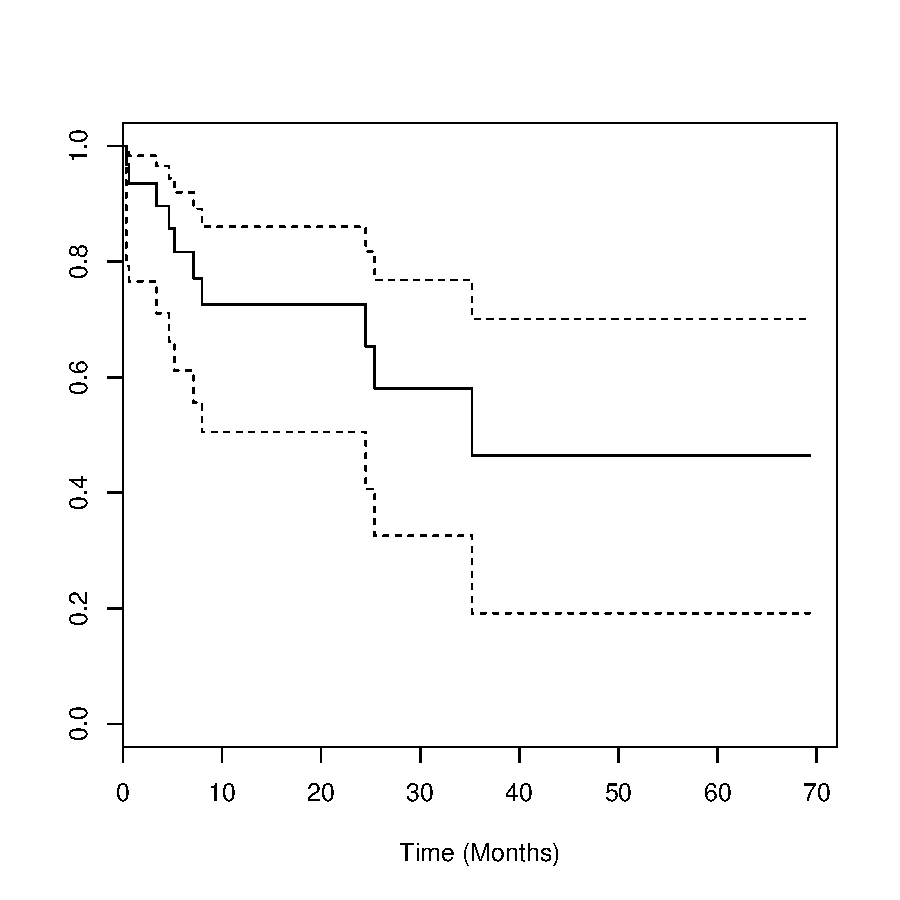
\includegraphics[width=0.8\textwidth]{Z:/projetstlouis/scripts/Rapport-figtrmsp.pdf}
\captionof{figure}{TRM in the group with progressive disease at graft}

\end{center}

CIF for relapse/progression  in the group with progressive disease at 6 months was 0.31 (95 \% 0.13 - 0.5)

CIF for relapse/progression  in the group with progressive disease at 1 years was 0.31 (95 \% 0.13 - 0.5), at 2 years  0.31 (95 \% 0.13 - 0.5).


\begin{center}
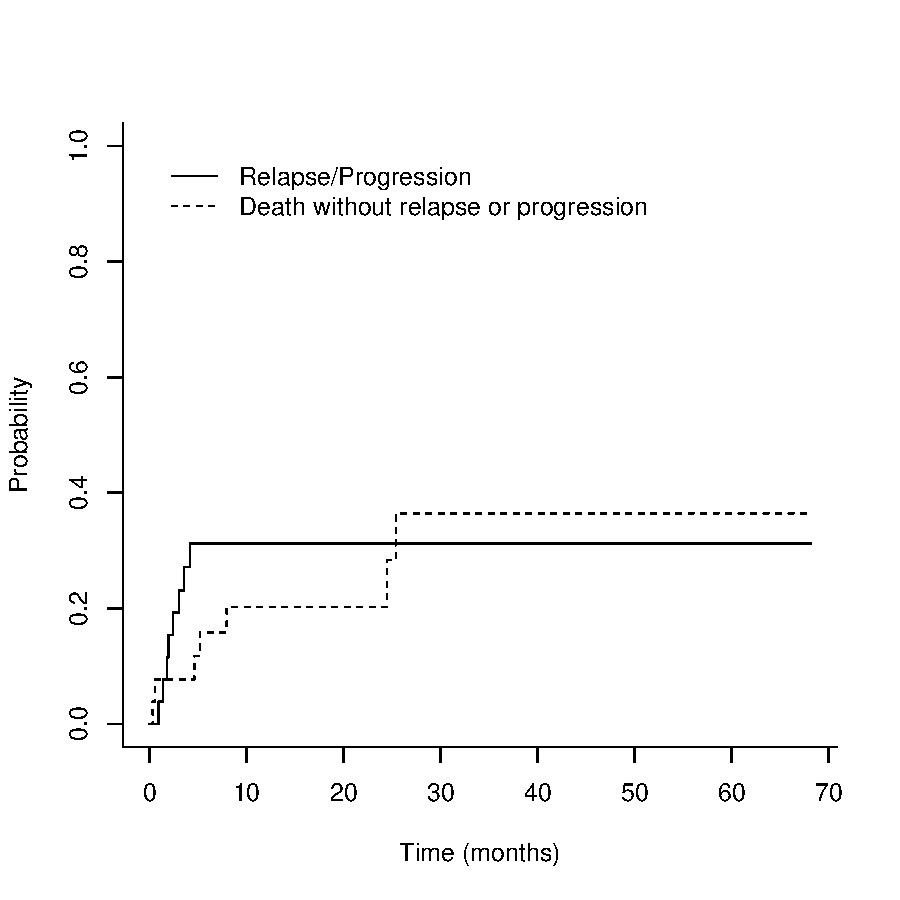
\includegraphics[width=0.8\textwidth]{Z:/projetstlouis/scripts/Rapport-figcifsp.pdf}
\captionof{figure}{CIF of relapse or progression and death without relapse or progression in the group with progressive disease at graft}

\end{center}





\subsection{CR1 analysis }

OS at 6 months was 0.77 (95 \% 0.67 - 0.84)
OS at 1 year was 0.68 (95 \% 0.57 - 0.77), was 0.62 (95 \% 0.51 - 0.72) at 2 years. OS at 4 years was 0.58 (95 \% 0.46 - 0.69).


\begin{center}
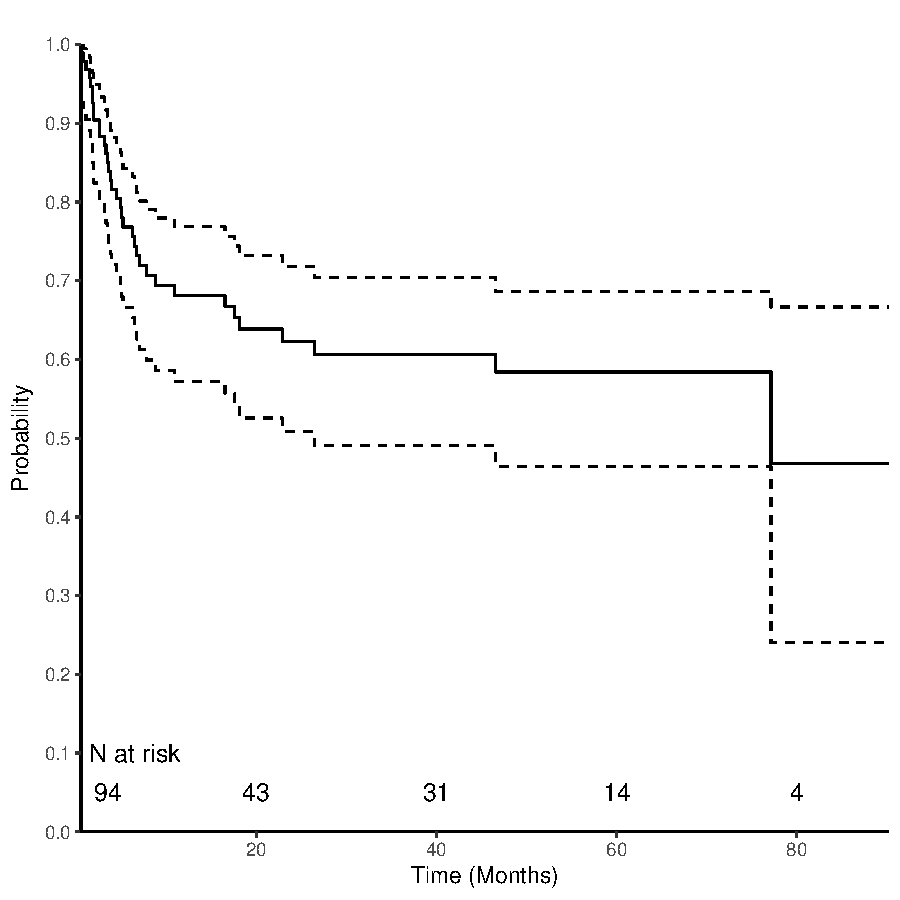
\includegraphics[width=0.8\textwidth]{Z:/projetstlouis/scripts/Rapport-figoscr1.pdf}
\captionof{figure}{OS in the CR1 group}

\end{center}




TRM at 6 months in the group with progressive disease was 0.15 (95 \% 0.24 - 0.09)

TRM at 1 year in the group with progressive disease was 0.23 (95 \% 0.34 - 0.15), was 0.27 (95 \% 0.38 - 0.18) at 2 years. TRM at 4 years was 0.27 (95 \% 0.38 - 0.18).

\begin{center}
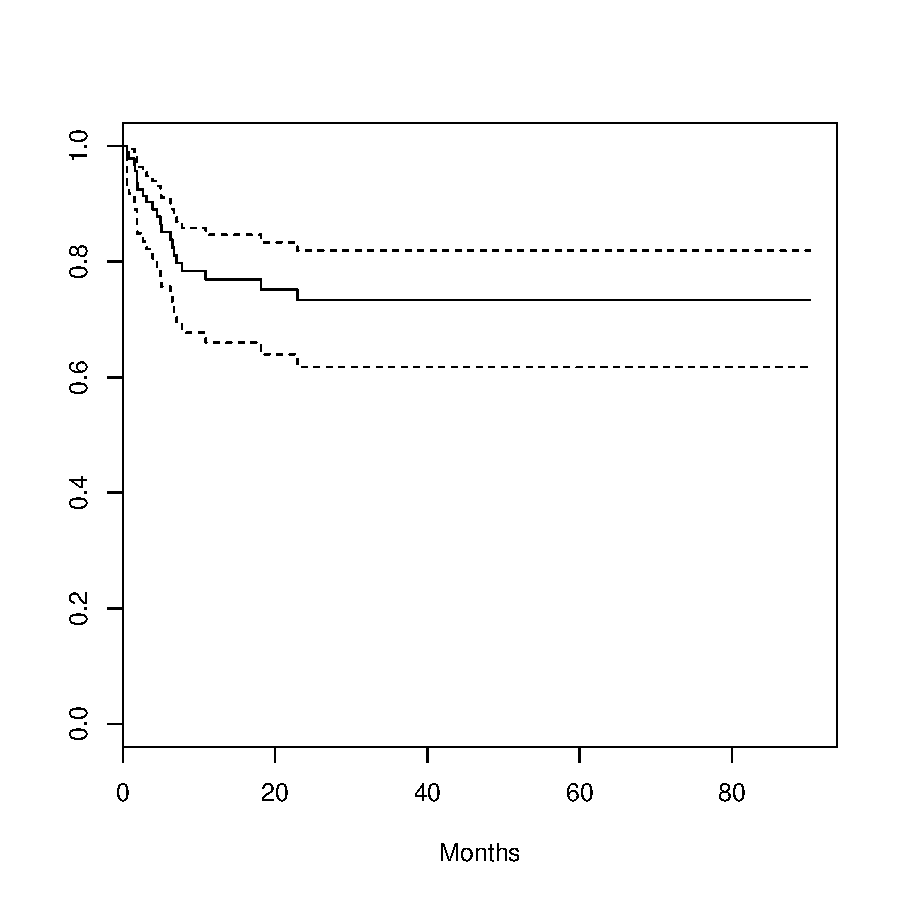
\includegraphics[width=0.8\textwidth]{Z:/projetstlouis/scripts/Rapport-figtrmcr1.pdf}
\captionof{figure}{TRM in the CR1 group}

\end{center}



CIF for relapse/progression  in the group with progressive disease at 6 months was 0.11 (95 \% 0.13 - 0.5).
CIF for relapse/progression  in the group with progressive disease at 1 years was 0.15 (95 \% 0.13 - 0.5), at 2 years  0.16 (95 \% 0.13 - 0.5).



\begin{center}
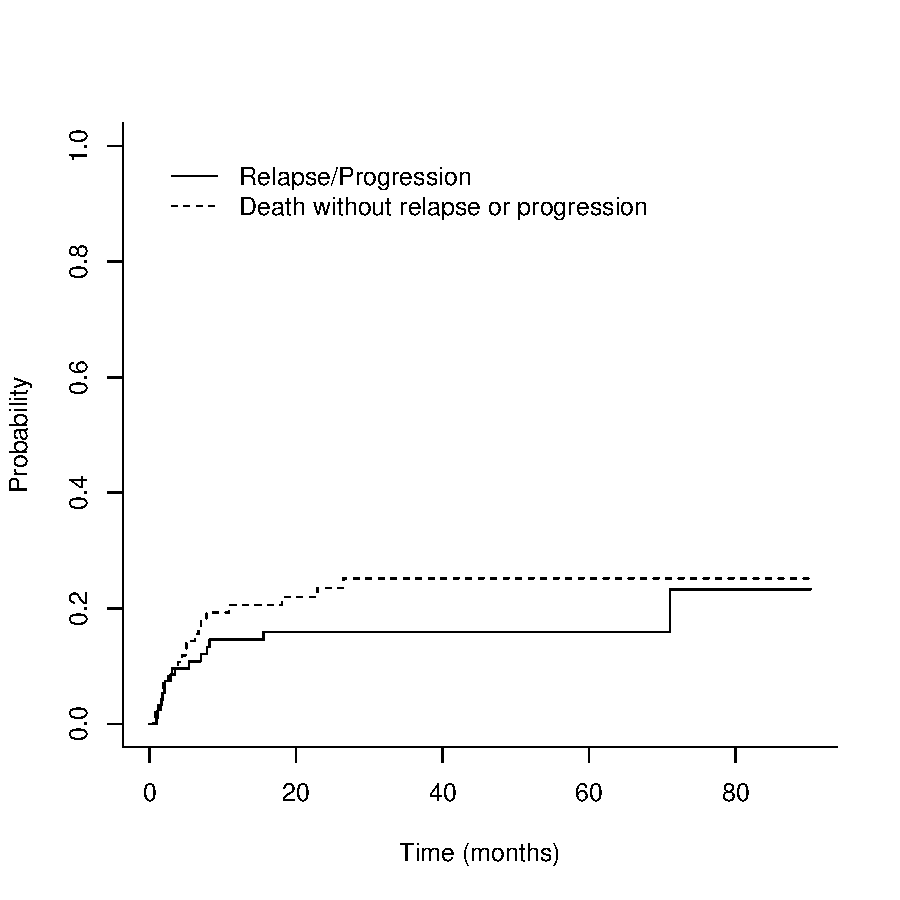
\includegraphics[width=0.8\textwidth]{Z:/projetstlouis/scripts/Rapport-figcifcr1.pdf}
\captionof{figure}{CIF of relapse or progression and death without relapse or progression in the CR1 group}

\end{center}






\pagebreak
\subsection{Survival analysis after a complete remisson post alloSCT}
245 patients whith a complete remission were included.


OS at 1 year was 0.74 (95 \% 0.68 - 0.8), was 0.7 (95 \% 0.64 - 0.76) at 2 years. OS at 4 years was 0.62 (95 \% 0.56 - 0.7).
\\
\begin{center}
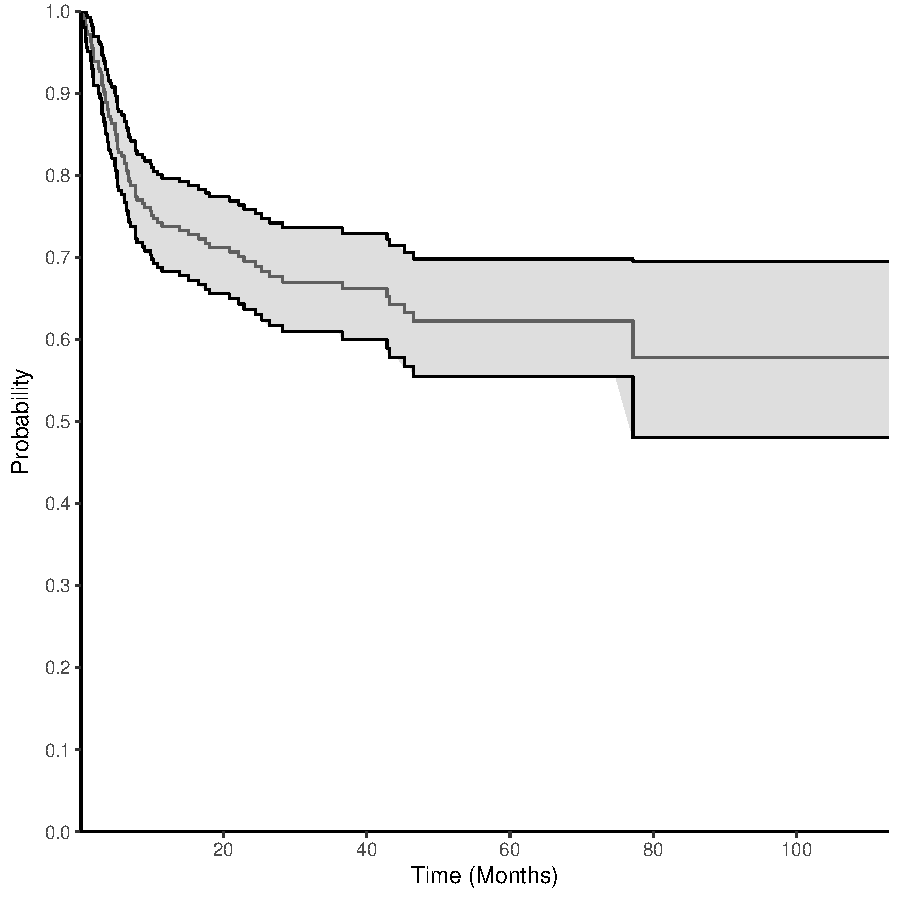
\includegraphics[width=0.5\textwidth]{Z:/projetstlouis/scripts/Rapport-figg.pdf}
\captionof{figure}{OS in patients with a complete remission post alloSCT}

\pagebreak
CIF for relapse at 1 year was 0.12 (95 \% 0.07 - 0.16), at 2 years  0.13 (95 \% 0.09 - 0.18). CIF for death without relapse  at 1 year was 0.19 (95 \% 0.14 - 0.24), at 2 years  0.22 (95 \% 0.17 - 0.28). 


\begin{center}
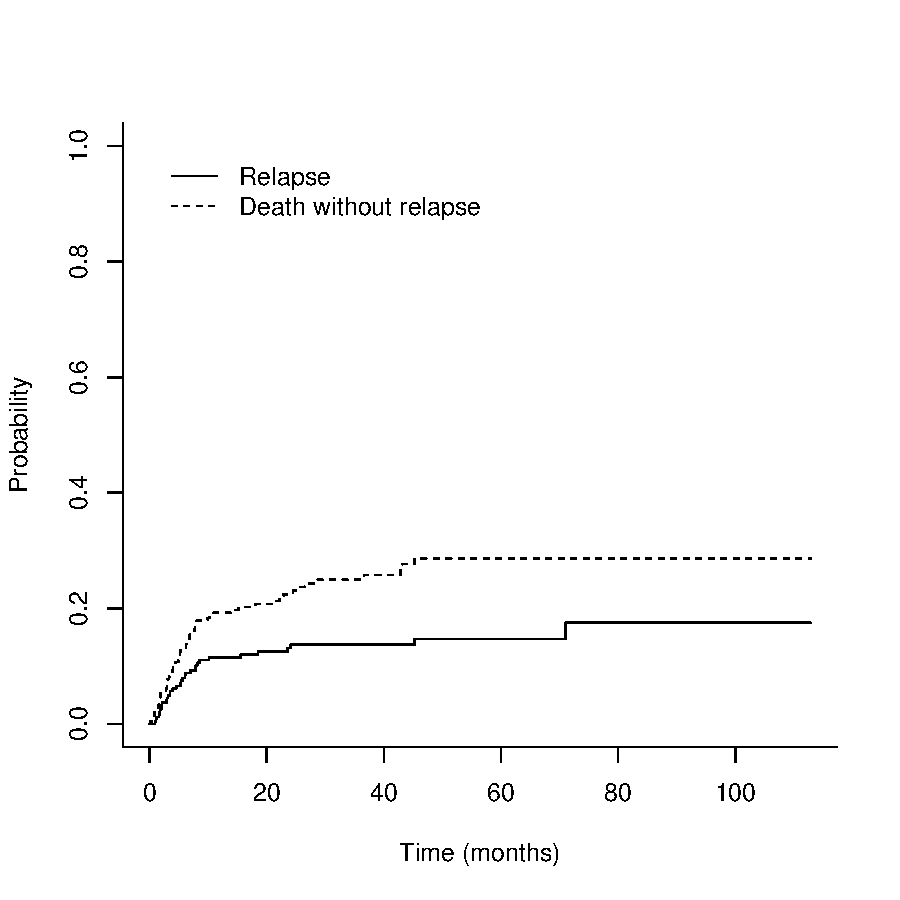
\includegraphics[width=0.8\textwidth]{Z:/projetstlouis/scripts/Rapport-fig7.pdf}
\captionof{figure}{CIF of relapse and death without relapse (in patients with a complete remission post alloSCT)}

\end{center}



%\end{center}
%\begin{center}
%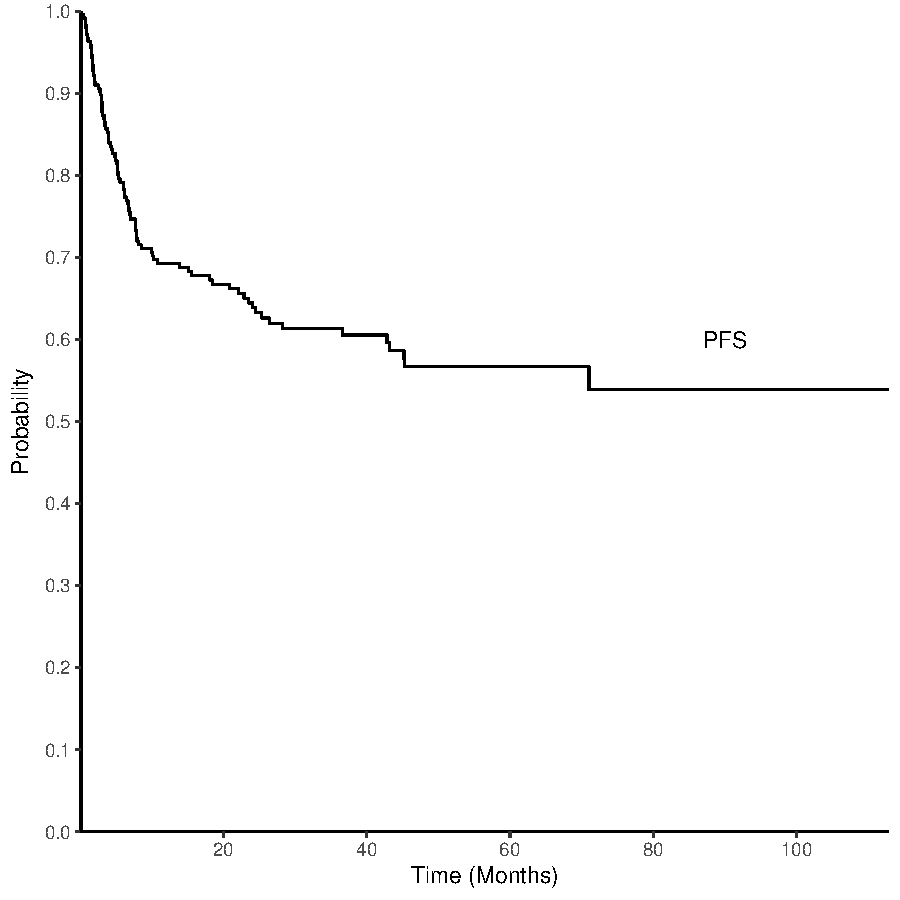
\includegraphics[width=0.5\textwidth]{Z:/projetstlouis/scripts/Rapport-figg2.pdf}
%\captionof{figure}{PFS in patients with a complete remission post alloSCT}

\end{center}
\begin{center} 
 
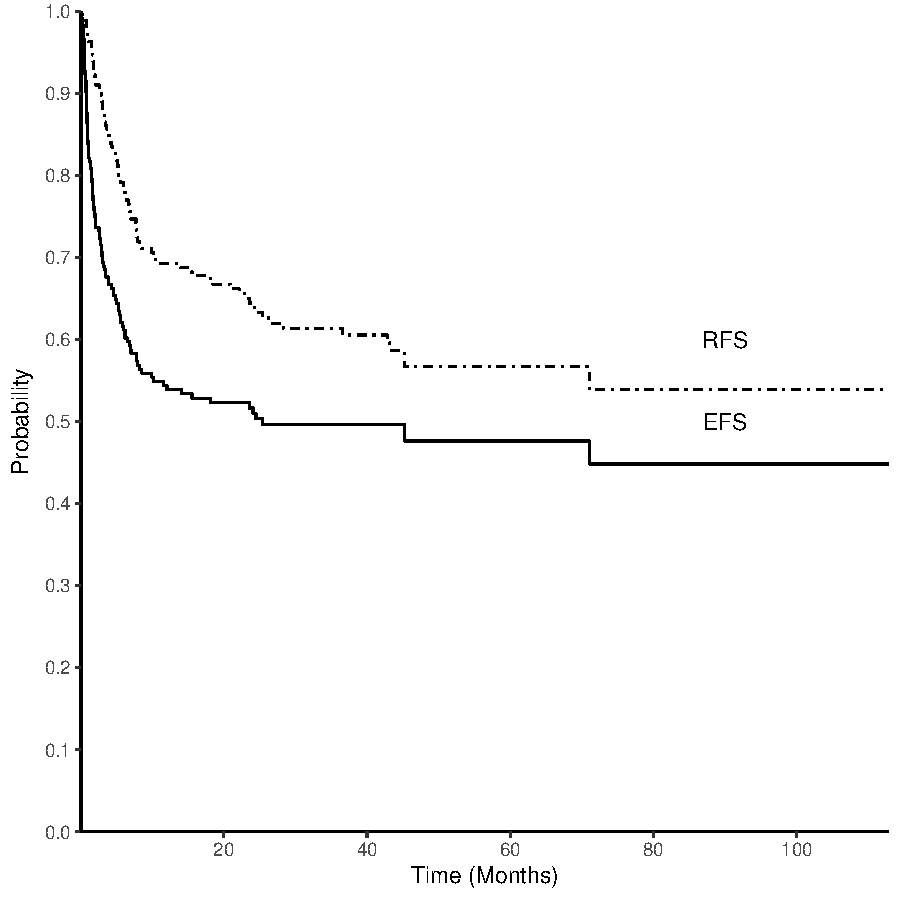
\includegraphics[width=0.5\textwidth]{Z:/projetstlouis/scripts/Rapport-xcube.pdf}
\captionof{figure}{RFS and EFS in patients with a complete remission post alloSCT}



%\end{center}



\pagebreak

\begin{cente0r}
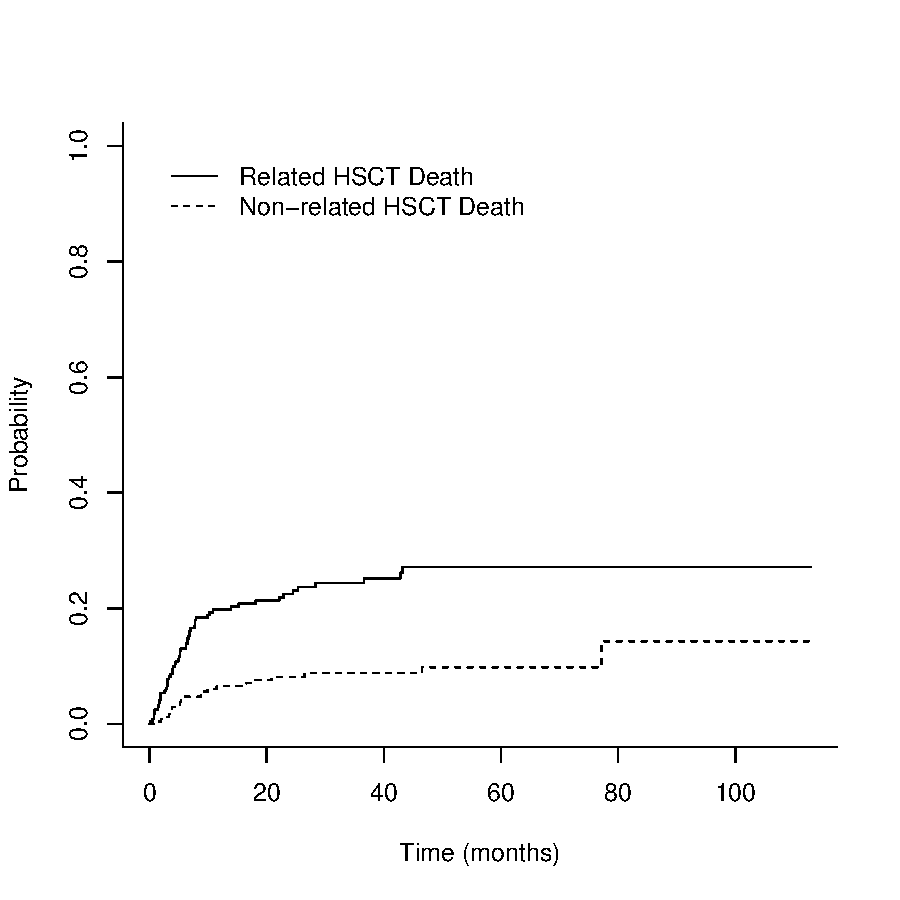
\includegraphics[width=0.8\textwidth]{Z:/projetstlouis/scripts/Rapport-fig99.pdf}
\captionof{figure}{CIF of Related HSCT Death and Non-related HSCT Death (in patients with a complete remission post alloSCT)}

\end{center}
\pagebreak
\begin{center}
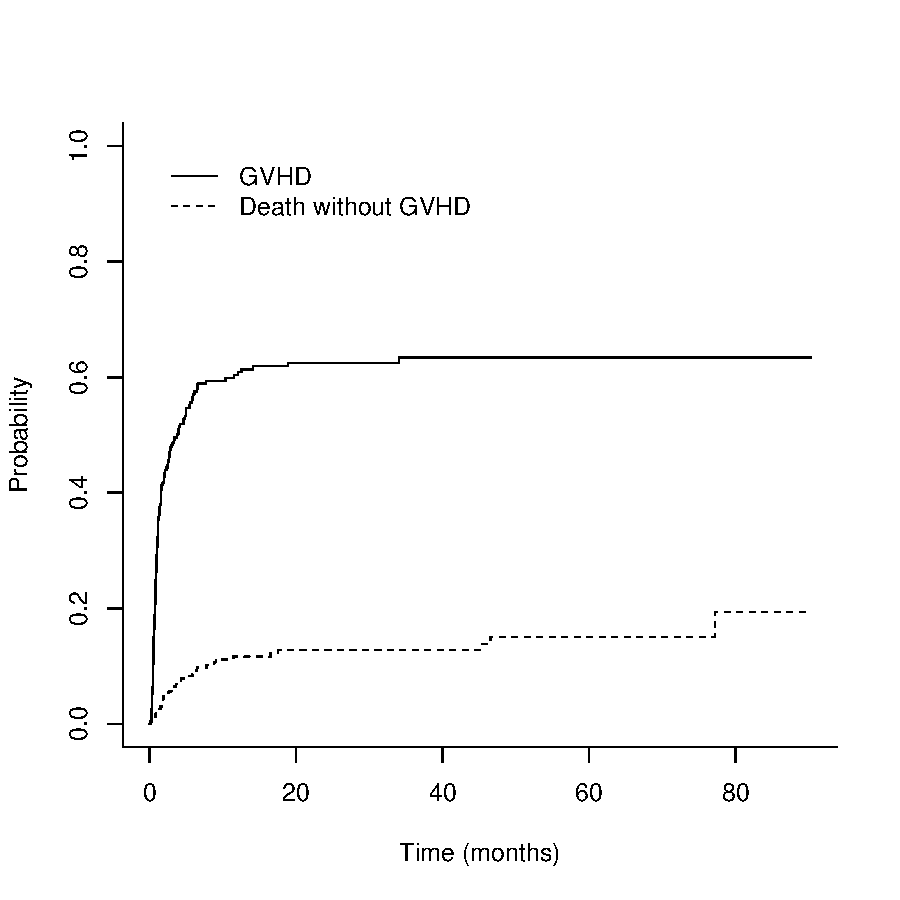
\includegraphics[width=0.8\textwidth]{Z:/projetstlouis/scripts/Rapport-fig98.pdf}
\captionof{figure}{CIF of GVHD and Death without GVHD (acute or chronic)(in patients with a complete remission post alloSCT)}

\end{center}

\begin{landscape}
%\subsection{Univariate Analysis}


\subsection{Survival analysis according to subtypes}

% latex table generated in R 3.4.4 by xtable 1.8-2 package
% Tue Jun 19 12:16:20 2018
\begin{longtable}{lllllllllll}
  \hline
histo & outcome & 1 an & BI 1 an & BS 1 an & 2 ans & BI 2 an & BS 2 an & 4 an & BI 4 an & BS 4 an \\ 
  \hline
NOS & os & 0.71 & 0.6 & 0.79 & 0.68 & 0.58 & 0.76 & 0.64 & 0.53 & 0.73 \\ 
  NOS & efs & 0.65 & 0.57 & 0.75 & 0.61 & 0.52 & 0.71 & 0.58 & 0.48 & 0.69 \\ 
  NOS & trm & 0.17 & 0.26 & 0.1 & 0.19 & 0.29 & 0.12 & 0.21 & 0.31 & 0.14 \\ 
  NOS & cif rechute/progression & 0.19 & 0.12 & 0.27 & 0.22 & 0.14 & 0.3 & 0.23 & 0.15 & 0.32 \\ 
  AITL & os & 0.73 & 0.62 & 0.82 & 0.66 & 0.54 & 0.76 & 0.52 & 0.37 & 0.65 \\ 
  AITL & efs & 0.7 & 0.6 & 0.81 & 0.61 & 0.51 & 0.74 & 0.49 & 0.38 & 0.65 \\ 
  AITL & trm & 0.24 & 0.35 & 0.16 & 0.29 & 0.41 & 0.2 & 0.43 & 0.59 & 0.3 \\ 
  AITL & cif rechute/progression & 0.1 & 0.04 & 0.17 & 0.12 & 0.05 & 0.2 & 0.12 & 0.05 & 0.2 \\ 
  ALCL ALK+ & os & 0.81 & 0.57 & 0.92 & 0.81 & 0.57 & 0.92 & 0.67 & 0.32 & 0.87 \\ 
  ALCL ALK+ & efs & 0.75 & 0.58 & 0.97 & 0.75 & 0.58 & 0.97 & 0.62 & 0.4 & 0.97 \\ 
  ALCL ALK+ & trm & 0.05 & 0.32 & 0.01 & 0.05 & 0.32 & 0.01 & 0.21 & 0.68 & 0.05 \\ 
  ALCL ALK+ & cif rechute/progression & 0.2 & 0.02 & 0.38 & 0.2 & 0.02 & 0.38 & 0.2 & 0.02 & 0.38 \\ 
  NK/T nasal & os & 0.5 & 0.25 & 0.71 & 0.5 & 0.25 & 0.71 & 0.5 & 0.25 & 0.71 \\ 
  NK/T nasal & efs & 0.44 & 0.25 & 0.76 & 0.44 & 0.25 & 0.76 & 0.44 & 0.25 & 0.76 \\ 
  NK/T nasal & trm & 0.29 & 0.61 & 0.12 & 0.29 & 0.61 & 0.12 & 0.29 & 0.61 & 0.12 \\ 
  NK/T nasal & cif rechute/progression &  &  &  &  &  &  &  &  &  \\ 
  HS & os & 0.56 & 0.23 & 0.79 & 0.56 & 0.23 & 0.79 & 0.56 & 0.23 & 0.79 \\ 
  HS & efs & 0.61 & 0.36 & 1 & 0.61 & 0.36 & 1 & 0.61 & 0.36 & 1 \\ 
  HS & trm & 0.44 & 0.77 & 0.21 & 0.44 & 0.77 & 0.21 & 0.44 & 0.77 & 0.21 \\ 
  HS & cif rechute/progression &  &  &  &  &  &  &  &  &  \\ 
  EATL & os & 0.67 & 0.05 & 0.95 & 0.67 & 0.05 & 0.95 & 0.67 & 0.05 & 0.95 \\ 
  EATL & efs & 0.67 & 0.3 & 1 & 0.67 & 0.3 & 1 & 0.67 & 0.3 & 1 \\ 
  EATL & trm & 0 &  &  & 0 &  &  & 0 &  &  \\ 
  EATL & cif rechute/progression &  &  &  &  &  &  &  &  &  \\ 
  Autres ALCL & os & 0.55 & 0.32 & 0.72 & 0.5 & 0.28 & 0.68 & 0.5 & 0.28 & 0.68 \\ 
  Autres ALCL & efs & 0.52 & 0.35 & 0.79 & 0.52 & 0.35 & 0.79 & 0.44 & 0.25 & 0.75 \\ 
  Autres ALCL & trm & 0.34 & 0.58 & 0.18 & 0.34 & 0.58 & 0.18 & 0.34 & 0.58 & 0.18 \\ 
  Autres ALCL & cif rechute/progression & 0.14 & -0.01 & 0.3 & 0.14 & -0.01 & 0.3 & 0.23 & 0.01 & 0.45 \\ 
   \hline
\hline
\caption{OS, EFS, TRM, CIF of relapse/progression} 
\label{tab:S}
\end{longtable}

\subsection{Survival analysis in front line patients n=284}

% latex table generated in R 3.4.4 by xtable 1.8-2 package
% Tue Jun 19 12:16:20 2018
\begin{longtable}{rlllllllllll}
  \hline
 & histo & outcome & 1 an & BI 1 an & BS 1 an & 2 ans & BI 2 an & BS 2 an & 4 an & BI 4 an & BS 4 an \\ 
  \hline
ost & 1 & os & 0.69 & 0.61 & 0.76 & 0.65 & 0.56 & 0.72 & 0.59 & 0.49 & 0.67 \\ 
  efst & 1 & efs & 0.62 & 0.55 & 0.71 & 0.59 & 0.51 & 0.68 & 0.55 & 0.47 & 0.65 \\ 
  trmt & 1 & trm & 0.22 & 0.3 & 0.15 & 0.24 & 0.32 & 0.17 & 0.25 & 0.34 & 0.18 \\ 
  rechutet & 1 & cif rechute/progression & 0.19 & 0.12 & 0.25 & 0.2 & 0.13 & 0.26 & 0.21 & 0.14 & 0.28 \\ 
   \hline
\hline
\caption{OS, EFS, TRM, CIF of relapse/progression} 
\label{tab:S1}
\end{longtable}



\subsection{Univariate Analysis and multivariate analysis }

% latex table generated in R 3.4.4 by xtable 1.8-2 package
% Tue Jun 19 12:16:20 2018
\begin{longtable}{llrlll}
  \hline
variable & Variable & HR & IC & pval & p \\ 
  \hline
Age at graft &  &  &  &  & 0.37 \\ 
   &  & 0.99 & [0.98 - 1.01] & 0.37 &  \\ 
  subtypes & NOS & 1.00 &  &  & 0.84 \\ 
   & AITL & 0.83 & [0.51 - 1.35] & 0.46 &  \\ 
   & ALCL & 1.25 & [0.73 - 2.14] & 0.42 &  \\ 
   & ATLL & 0.94 & [0.4 - 2.21] & 0.88 &  \\ 
   & NK/T nasal & 0.78 & [0.31 - 1.96] & 0.59 &  \\ 
   & Others & 0.94 & [0.42 - 2.1] & 0.88 &  \\ 
  Delay between diag and allo SCT > 12 mo & NO & 1.00 &  &  & 0.16 \\ 
   & Yes & 1.31 & [0.9 - 1.92] & 0.16 &  \\ 
  Stage at diagnosis & I & 1.00 &  &  & 0.67 \\ 
   & II & 1.04 & [0.28 - 3.86] & 0.96 &  \\ 
   & III & 1.65 & [0.57 - 4.81] & 0.36 &  \\ 
   & IV & 1.35 & [0.49 - 3.74] & 0.56 &  \\ 
  Disease status at transplant & CR & 1.00 &  &  & 0.61 \\ 
   & PR & 1.17 & [0.77 - 1.79] & 0.47 &  \\ 
   & PD & 0.85 & [0.45 - 1.61] & 0.61 &  \\ 
  Karnofsky score & 100 & 1.00 &  &  & 0.88 \\ 
   & Unable to carry on normal activity & 1.23 & [0.54 - 2.78] & 0.62 &  \\ 
   & 90-80 & 1.01 & [0.66 - 1.54] & 0.97 &  \\ 
  First graft relapse & No & 1.00 &  &  & 0.82 \\ 
   & No previous graft & 1.02 & [0.54 - 1.93] & 0.94 &  \\ 
   & Yes & 0.88 & [0.42 - 1.83] & 0.73 &  \\ 
  No of lines before alloSCT & >2 & 1.00 &  &  & 0.58 \\ 
   & 1 or 2 & 1.12 & [0.74 - 1.7] & 0.58 &  \\ 
  HLA match & HLA mismatched & 1.00 &  &  & 0.99 \\ 
   & HLA matched & 1.00 & [0.62 - 1.63] & 0.99 &  \\ 
  Sex of donnor-patient & Others & 1.00 &  &  & 0.48 \\ 
   & F/M & 0.85 & [0.54 - 1.34] & 0.49 &  \\ 
  CMV serostatus of donnor patient & neg/neg & 1.00 &  &  & 0.003 \\ 
   & Others & 1.92 & [1.22 - 3.04] & 0.005 &  \\ 
  Source of stem cells & BM & 1.00 &  &  & 0.57 \\ 
   & CB & 0.92 & [0.42 - 2.01] & 0.84 &  \\ 
   & PB & 1.22 & [0.72 - 2.06] & 0.46 &  \\ 
  Conditionning intensity & MAC & 1.00 &  &  & 0.016 \\ 
   & NMA & 0.33 & [0.13 - 0.84] & 0.020 &  \\ 
   & RIC & 0.70 & [0.47 - 1.03] & 0.071 &  \\ 
  Depletion & No & 1.00 &  &  & 0.80 \\ 
   & Partial T depletion & 0.79 & [0.11 - 5.64] & 0.81 &  \\ 
  Agvhd grade 3-4 &  &  &  &  & <0.0001 \\ 
   &  & 2.82 & [1.78 - 4.47] & <0.0001 &  \\ 
  Cgvhd &  &  &  &  & 0.17 \\ 
   &  & 1.44 & [0.86 - 2.41] & 0.16 &  \\ 
   \hline
\hline
\caption{Univariate analysis of 5 years OS survival} 
\label{tab:uos}
\end{longtable}


% latex table generated in R 3.3.2 by xtable 1.8-2 package
% Fri May 26 14:16:17 2017
% latex table generated in R 3.4.4 by xtable 1.8-2 package
% Tue Jun 19 12:16:20 2018
\begin{longtable}{llll}
  \hline
V1 & Variable & HR (95\%CI) & \emph{P} \\ 
  \hline
Agvhd & Grade 3-4 Agvhd & 2.39 (1.42--4.04) & 0.001 \\ 
  Sex of donnor-patient & F/M & 1.48 (0.92--2.36) & 0.10 \\ 
  Disease status at transplant & PR & 0.72 (0.43--1.22) & 0.22 \\ 
   & PD & 1.40 (0.72--2.73) & 0.31 \\ 
  Karnofsky score & Unable to carry on normal activity & 3.37 (1.38--8.24) & 0.008 \\ 
   & 90-80 & 2.20 (1.29--3.76) & 0.004 \\ 
  Stem cell source & CB & 2.42 (0.84--6.95) & 0.10 \\ 
   & PB & 0.85 (0.49--1.49) & 0.57 \\ 
  Agvhd &  & 0.77 (0.46--1.30) & 0.33 \\ 
  Sex of donnor-patient &  & 1.43 (0.60--3.40) & 0.42 \\ 
   \hline
\hline
\caption{Multivariate analysis of 5 years OS (stratified on the delay between diagnosis and alloSCT)} 
\label{tab:uos}
\end{longtable}\end{landscape}

\begin{landscape}
% latex table generated in R 3.4.4 by xtable 1.8-2 package
% Tue Jun 19 12:16:20 2018
\begin{longtable}{llrlll}
  \hline
variable & Variable & HR & IC & pval & p \\ 
  \hline
Age at graft &  &  &  &  & 0.62 \\ 
   &  & 1.00 & [0.98 - 1.01] & 0.61 &  \\ 
  subtypes & NOS & 1.00 &  &  & 0.33 \\ 
   & AITL & 0.78 & [0.51 - 1.17] & 0.23 &  \\ 
   & ALCL & 1.23 & [0.77 - 1.98] & 0.38 &  \\ 
   & ATLL & 0.77 & [0.35 - 1.69] & 0.51 &  \\ 
   & NK/T nasal & 0.55 & [0.22 - 1.37] & 0.20 &  \\ 
   & Others & 0.72 & [0.34 - 1.51] & 0.39 &  \\ 
  Delay between diag and allo SCT & NO & 1.00 &  &  & 0.73 \\ 
   & Yes & 0.94 & [0.68 - 1.31] & 0.73 &  \\ 
  Stage at diagnosis & I & 1.00 &  &  & 0.79 \\ 
   & II & 1.05 & [0.34 - 3.25] & 0.94 &  \\ 
   & III & 1.44 & [0.59 - 3.53] & 0.43 &  \\ 
   & IV & 1.34 & [0.58 - 3.1] & 0.49 &  \\ 
  Disease status at transplant & CR & 1.00 &  &  & 0.15 \\ 
   & PR & 1.21 & [0.84 - 1.75] & 0.31 &  \\ 
   & PD & 0.65 & [0.35 - 1.22] & 0.18 &  \\ 
  Karnofsky score & 100 & 1.00 &  &  & 0.48 \\ 
   & Unable to carry on normal activity & 1.38 & [0.69 - 2.73] & 0.36 &  \\ 
   & 90-80 & 0.91 & [0.63 - 1.31] & 0.60 &  \\ 
  First graft relapse & No & 1.00 &  &  & 0.42 \\ 
   & No previous graft & 0.89 & [0.51 - 1.54] & 0.68 &  \\ 
   & Yes & 1.16 & [0.63 - 2.13] & 0.63 &  \\ 
  No of lines before alloSCT & >2 & 1.00 &  &  & 0.93 \\ 
   & 1 or 2 & 0.98 & [0.68 - 1.42] & 0.93 &  \\ 
  HLA match & HLA mismatched & 1.00 &  &  & 0.66 \\ 
   & HLA matched & 0.91 & [0.59 - 1.39] & 0.66 &  \\ 
  Sex of donnor-patient & Others & 1.00 &  &  & 0.44 \\ 
   & F/M & 0.86 & [0.58 - 1.27] & 0.44 &  \\ 
  CMV serostatus of donnor patient & neg/neg & 1.00 &  &  & 0.40 \\ 
   & Others & 1.17 & [0.81 - 1.67] & 0.41 &  \\ 
  Source of stem cells & BM & 1.00 &  &  & 0.83 \\ 
   & CB & 0.87 & [0.45 - 1.67] & 0.67 &  \\ 
   & PB & 1.03 & [0.66 - 1.6] & 0.90 &  \\ 
  Conditionning intensity & MAC & 1.00 &  &  & 0.35 \\ 
   & NMA & 0.76 & [0.4 - 1.44] & 0.40 &  \\ 
   & RIC & 0.78 & [0.55 - 1.11] & 0.16 &  \\ 
  Depletion & No & 1.00 &  &  & 0.30 \\ 
   & Partial T depletion & 0.41 & [0.06 - 2.93] & 0.37 &  \\ 
   \hline
\hline
\caption{Univariate analysis of 5 years GRFS} 
\label{tab:uos}
\end{longtable}


% latex table generated in R 3.4.4 by xtable 1.8-2 package
% Tue Jun 19 12:16:21 2018
\begin{longtable}{llll}
  \hline
V1 & Variable & HR (95\%CI) & \emph{P} \\ 
  \hline
Subtypes & AITL & 0.78 (0.51--1.18) & 0.23 \\ 
   & ALCL & 1.30 (0.81--2.09) & 0.28 \\ 
   & ATLL & 0.77 (0.35--1.72) & 0.53 \\ 
   & NK/T nasal & 0.53 (0.21--1.33) & 0.18 \\ 
   & Others & 0.68 (0.32--1.44) & 0.31 \\ 
  Disease status at transplant & PR & 1.23 (0.84--1.80) & 0.29 \\ 
   & PD & 0.63 (0.34--1.20) & 0.16 \\ 
  Source of stem cells & CB & 0.93 (0.47--1.84) & 0.83 \\ 
   & PB & 1.01 (0.65--1.58) & 0.96 \\ 
   \hline
\hline
\caption{Multivariate analysis of 5 years GRFS} 
\label{tab:uos}
\end{longtable}\end{landscape}


\begin{landscape}
% latex table generated in R 3.4.4 by xtable 1.8-2 package
% Tue Jun 19 12:16:21 2018
\begin{longtable}{llrlll}
  \hline
variable & Variable & HR & IC & pval & p \\ 
  \hline
Age at graft &  &  &  &  & 0.72 \\ 
   &  & 1.00 & [0.98 - 1.01] & 0.72 &  \\ 
  subtypes & NOS & 1.00 &  &  & 0.72 \\ 
   & AITL & 0.89 & [0.57 - 1.38] & 0.61 &  \\ 
   & ALCL & 1.08 & [0.63 - 1.83] & 0.79 &  \\ 
   & ATLL & 0.74 & [0.32 - 1.73] & 0.49 &  \\ 
   & NK/T nasal & 0.51 & [0.18 - 1.41] & 0.19 &  \\ 
   & Others & 0.85 & [0.38 - 1.88] & 0.69 &  \\ 
  Delay between diag and allo SCT > 12 mo & NO & 1.00 &  &  & 0.85 \\ 
   & Yes & 1.04 & [0.72 - 1.49] & 0.85 &  \\ 
  Stage at diagnosis & I & 1.00 &  &  & 0.12 \\ 
   & II & 0.54 & [0.13 - 2.28] & 0.40 &  \\ 
   & III & 1.80 & [0.69 - 4.72] & 0.23 &  \\ 
   & IV & 1.28 & [0.51 - 3.2] & 0.59 &  \\ 
  Disease status at transplant & CR & 1.00 &  &  & 0.50 \\ 
   & PR & 1.12 & [0.75 - 1.68] & 0.58 &  \\ 
   & PD & 0.76 & [0.4 - 1.43] & 0.39 &  \\ 
  Karnofsky score & 100 & 1.00 &  &  & 0.60 \\ 
   & Unable to carry on normal activity & 1.32 & [0.64 - 2.73] & 0.45 &  \\ 
   & 90-80 & 0.91 & [0.61 - 1.37] & 0.67 &  \\ 
  First graft relapse & No & 1.00 &  &  & 0.74 \\ 
   & No previous graft & 0.80 & [0.45 - 1.45] & 0.47 &  \\ 
   & Yes & 0.89 & [0.46 - 1.73] & 0.73 &  \\ 
  No of lines before alloSCT & >2 & 1.00 &  &  & 0.60 \\ 
   & 1 or 2 & 1.11 & [0.74 - 1.66] & 0.60 &  \\ 
  HLA match & HLA mismatched & 1.00 &  &  & 0.80 \\ 
   & HLA matched & 0.94 & [0.59 - 1.5] & 0.80 &  \\ 
  Sex of donnor-patient & Others & 1.00 &  &  & 0.38 \\ 
   & F/M & 0.82 & [0.53 - 1.27] & 0.38 &  \\ 
  CMV serostatus of donnor patient & neg/neg & 1.00 &  &  & 0.057 \\ 
   & Others & 1.47 & [0.98 - 2.2] & 0.064 &  \\ 
  Source of stem cells & BM & 1.00 &  &  & 0.80 \\ 
   & CB & 1.17 & [0.58 - 2.36] & 0.67 &  \\ 
   & PB & 1.18 & [0.72 - 1.94] & 0.51 &  \\ 
  Conditionning intensity & MAC & 1.00 &  &  & 0.097 \\ 
   & NMA & 0.51 & [0.24 - 1.08] & 0.077 &  \\ 
   & RIC & 0.74 & [0.5 - 1.07] & 0.11 &  \\ 
  Depletion & No & 1.00 &  &  & 0.62 \\ 
   & Partial T depletion & 0.63 & [0.09 - 4.54] & 0.65 &  \\ 
  Agvhd grade 3-4 &  &  &  &  & 0.004 \\ 
   &  & 2.09 & [1.31 - 3.34] & 0.002 &  \\ 
  Cgvhd &  &  &  &  & 0.10 \\ 
   &  & 1.56 & [0.93 - 2.64] & 0.094 &  \\ 
   \hline
\hline
\caption{Univariate analysis of 5 years EFS} 
\label{tab:uos}
\end{longtable}
% latex table generated in R 3.4.4 by xtable 1.8-2 package
% Tue Jun 19 12:16:21 2018
\begin{longtable}{llll}
  \hline
V1 & Variable & HR (95\%CI) & \emph{P} \\ 
  \hline
N of lines & 1 or 2 & 0.74 (0.49--1.12) & 0.15 \\ 
  Karnofsky score & Unable to carry on normal activity & 1.28 (0.44--3.76) & 0.65 \\ 
   & 90-80 & 2.27 (1.43--3.61) & 0.0005 \\ 
  Cell source & CB & 1.96 (0.96--4.01) & 0.065 \\ 
   & PB & 1.02 (0.59--1.77) & 0.95 \\ 
  N of lines &  & 1.68 (0.96--2.93) & 0.068 \\ 
  Karnofsky score &  & 1.95 (1.15--3.29) & 0.013 \\ 
   \hline
\hline
\caption{Multivariate analysis of 5 years EFS} 
\label{tab:uos}
\end{longtable}\end{landscape}



\begin{landscape}
% latex table generated in R 3.4.4 by xtable 1.8-2 package
% Tue Jun 19 12:16:21 2018
\begin{longtable}{llrlll}
  \hline
variable & Variable & HR & IC & pval & p \\ 
  \hline
Age at graft &  &  &  &  & 0.017 \\ 
   &  & 1.02 & [1 - 1.05] & 0.022 &  \\ 
  subtypes & NOS & 1.00 &  &  & 0.28 \\ 
   & AITL & 1.87 & [1.03 - 3.38] & 0.039 &  \\ 
   & ALCL & 1.20 & [0.54 - 2.64] & 0.66 &  \\ 
   & ATLL & 1.31 & [0.39 - 4.43] & 0.67 &  \\ 
   & NK/T nasal & 1.68 & [0.57 - 4.94] & 0.35 &  \\ 
   & Others & 2.42 & [0.97 - 6.06] & 0.059 &  \\ 
  Delay between diag and allo SCT > 12 mo & NO & 1.00 &  &  & 0.76 \\ 
   & Yes & 0.93 & [0.57 - 1.5] & 0.76 &  \\ 
  Stage at diagnosis & I & 1.00 &  &  & 0.47 \\ 
   & II & 0.48 & [0.08 - 2.9] & 0.43 &  \\ 
   & III & 1.31 & [0.38 - 4.54] & 0.67 &  \\ 
   & IV & 0.93 & [0.28 - 3.04] & 0.90 &  \\ 
  Disease status at transplant & CR & 1.00 &  &  & 0.33 \\ 
   & PR & 0.86 & [0.48 - 1.53] & 0.60 &  \\ 
   & PD & 1.59 & [0.79 - 3.18] & 0.19 &  \\ 
  Karnofsky score & 100 & 1.00 &  &  & 0.040 \\ 
   & Unable to carry on normal activity & 2.30 & [0.75 - 6.98] & 0.14 &  \\ 
   & 90-80 & 2.04 & [1.12 - 3.73] & 0.020 &  \\ 
  First graft relapse & No & 1.00 &  &  & 0.014 \\ 
   & No previous graft & 4.33 & [1.05 - 17.9] & 0.043 &  \\ 
   & Yes & 5.57 & [1.3 - 23.76] & 0.020 &  \\ 
  No of lines before alloSCT & >2 & 1.00 &  &  & 0.055 \\ 
   & 1 or 2 & 0.61 & [0.37 - 1] & 0.052 &  \\ 
  HLA match & HLA mismatched & 1.00 &  &  & 0.46 \\ 
   & HLA matched & 0.80 & [0.44 - 1.43] & 0.45 &  \\ 
  Sex of donnor-patient & Others & 1.00 &  &  & 0.026 \\ 
   & F/M & 1.80 & [1.09 - 2.98] & 0.022 &  \\ 
  CMV serostatus of donnor patient & neg/neg & 1.00 &  &  & 0.99 \\ 
   & Others & 1.00 & [0.6 - 1.69] & 0.99 &  \\ 
  Source of stem cells & BM & 1.00 &  &  & 0.21 \\ 
   & CB & 1.29 & [0.57 - 2.91] & 0.54 &  \\ 
   & PB & 0.71 & [0.39 - 1.31] & 0.27 &  \\ 
  Conditionning intensity & MAC & 1.00 &  &  & 0.29 \\ 
   & NMA & 1.79 & [0.83 - 3.85] & 0.14 &  \\ 
   & RIC & 1.38 & [0.79 - 2.43] & 0.26 &  \\ 
  Depletion & No & 1.00 &  &  & 0.92 \\ 
   & Partial T depletion & 0.90 & [0.12 - 6.49] & 0.92 &  \\ 
   \hline
\hline
\caption{Univariate analysis of 5 years cause specific mortality : HSCT related } 
\label{tab:uos}
\end{longtable}


% latex table generated in R 3.4.4 by xtable 1.8-2 package
% Tue Jun 19 12:16:21 2018
\begin{longtable}{llll}
  \hline
V1 & Variable & HR (95\%CI) & \emph{P} \\ 
  \hline
Sex of donnor-patient & F/M & 1.87 (1.07--3.28) & 0.027 \\ 
  Karnofsky score & Unable to carry on normal activity & 2.52 (0.82--7.78) & 0.11 \\ 
   & 90-80 & 2.03 (1.08--3.83) & 0.029 \\ 
  Age at graft &  & 1.02 (1.00--1.04) & 0.084 \\ 
   \hline
\hline
\caption{Multivariate analysis of 5 years cause specific mortality : HSCT related (stratified on numbers of lines before alloSCT)} 
\label{tab:uos}
\end{longtable}\end{landscape}

%\subsection{Score de propension}

% latex table generated in R 3.4.4 by xtable 1.8-2 package
% Tue Jun 19 12:16:21 2018
\begin{longtable}{lrlll}
  \hline
Variable & HR & IC & pval & p \\ 
  \hline
MAC &  &  &  & 0.83 \\ 
  RIC/NMA & 0.89 & [0.3 - 2.62] & 0.83 &  \\ 
   \hline
\hline
\caption{Propensity score for 5 years OS} 
\label{label=tab:spos}
\end{longtable}

% latex table generated in R 3.4.4 by xtable 1.8-2 package
% Tue Jun 19 12:16:21 2018
\begin{longtable}{lrlll}
  \hline
Variable & HR & IC & pval & p \\ 
  \hline
MAC &  &  &  & 0.96 \\ 
  RIC/NMA & 0.98 & [0.41 - 2.33] & 0.96 &  \\ 
   \hline
\hline
\caption{Propensity score for 5 years EFS} 
\label{label=tab:spefs}
\end{longtable}

% latex table generated in R 3.4.4 by xtable 1.8-2 package
% Tue Jun 19 12:16:21 2018
\begin{longtable}{lrlll}
  \hline
Variable & HR & IC & pval & p \\ 
  \hline
MAC &  &  &  & 0.22 \\ 
  RIC/NMA & 0.45 & [0.12 - 1.65] & 0.23 &  \\ 
   \hline
\hline
\caption{Propensity score for 5 years HCST related death} 
\label{label=tab:tcspsp}
\end{longtable}
% latex table generated in R 3.4.4 by xtable 1.8-2 package
% Tue Jun 19 12:16:21 2018
\begin{longtable}{llll}
  \hline
Variables & HR & IC & pval \\ 
  \hline
MAC & 1 &  &  \\ 
  RIC/NMA & 2.08 & [ 0.64 - 6.74 ] &  0.22 \\ 
   \hline
\hline
\caption{Propensity score for 5 years relapse relapse (competitve risks)} 
\label{label=tab:tgreffematchitp}
\end{longtable}

\end{document}
